%!TEX root = ../dokumentation.tex

\section{Prototyping Stufe 1}
\subsection{Content Model}
\subsection{Abstract Prototype1}

\begin{figure}[H]
\centering
\hfill
\subfloat[aktionAuswahlen \label{pic:aktionAuswahlen}]{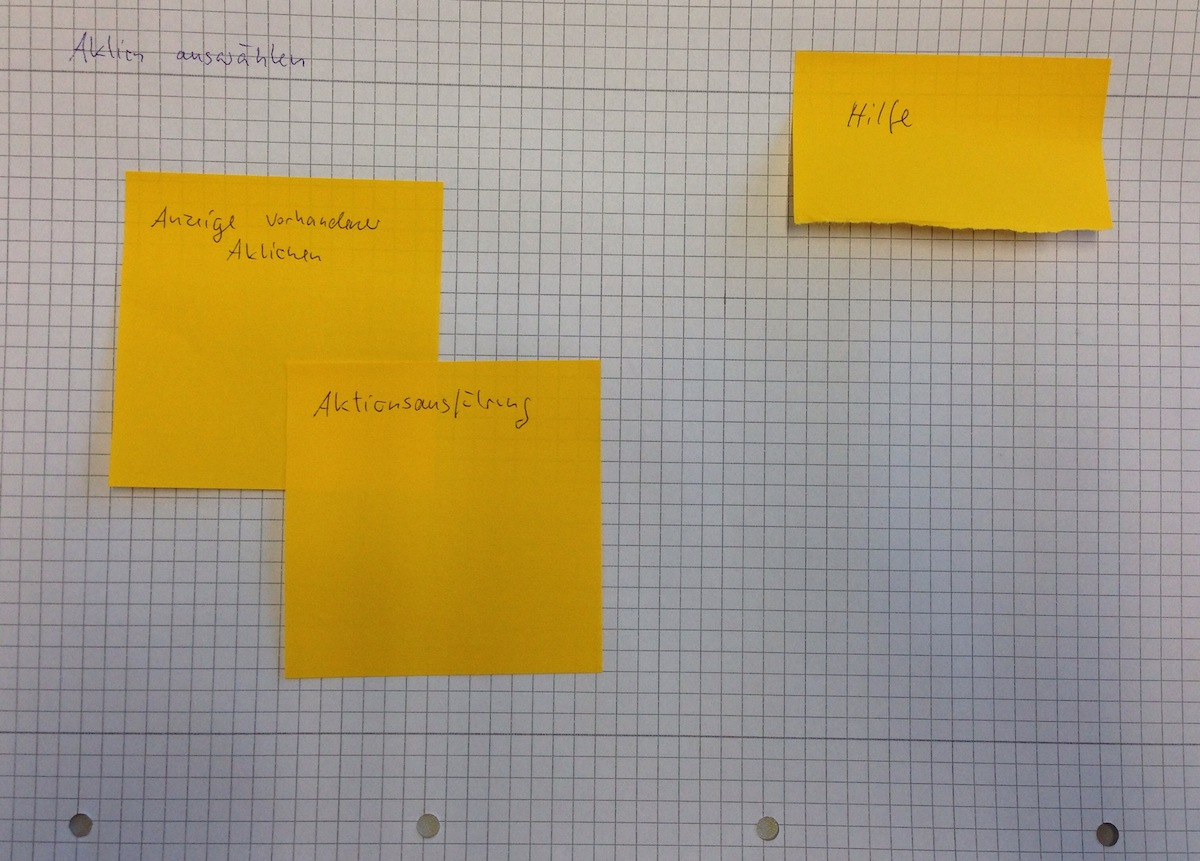
\includegraphics[width=.5\textwidth]{./images/abstract/version1/aktionAuswaehlen.JPG}}
\hfill % alternativ auch \hspace{1cm} für genaue Angaben
\subfloat[aktionBestaetigen \label{pic:aktionBestaetigen}]{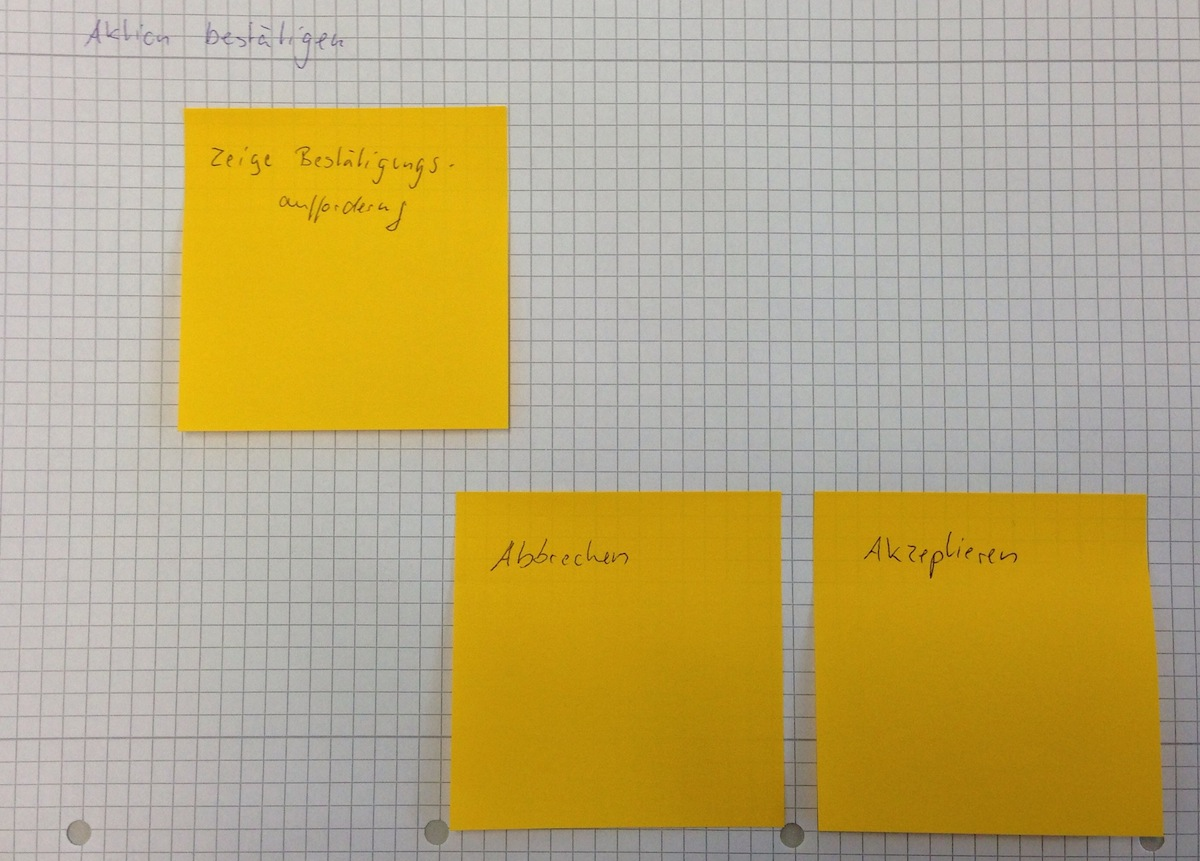
\includegraphics[width=.5\textwidth]{./images/abstract/version1/aktionBestaetigen.JPG}}
\hfill %
\caption{Interface Con. AP1: aktionAuswahlen und aktionBestaetigen }
\label{interfaceContents1}
\end{figure}

Beschreibung

\begin{figure}[H]
\centering
\hfill
\subfloat[ausloggen \label{pic:ausloggen}]{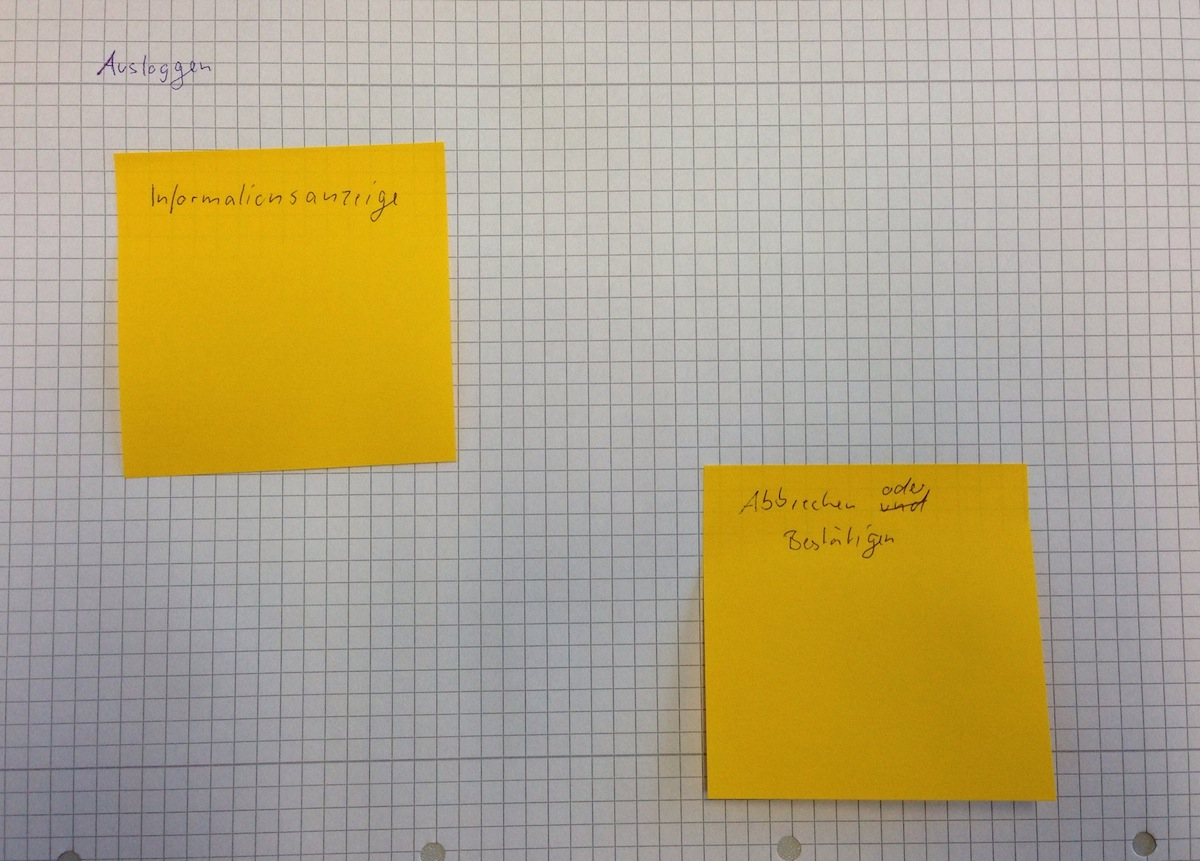
\includegraphics[width=.5\textwidth]{./images/abstract/version1/ausloggen.JPG}}
\hfill % alternativ auch \hspace{1cm} für genaue Angaben
\subfloat[bewerteUser \label{pic:bewerteUser}]{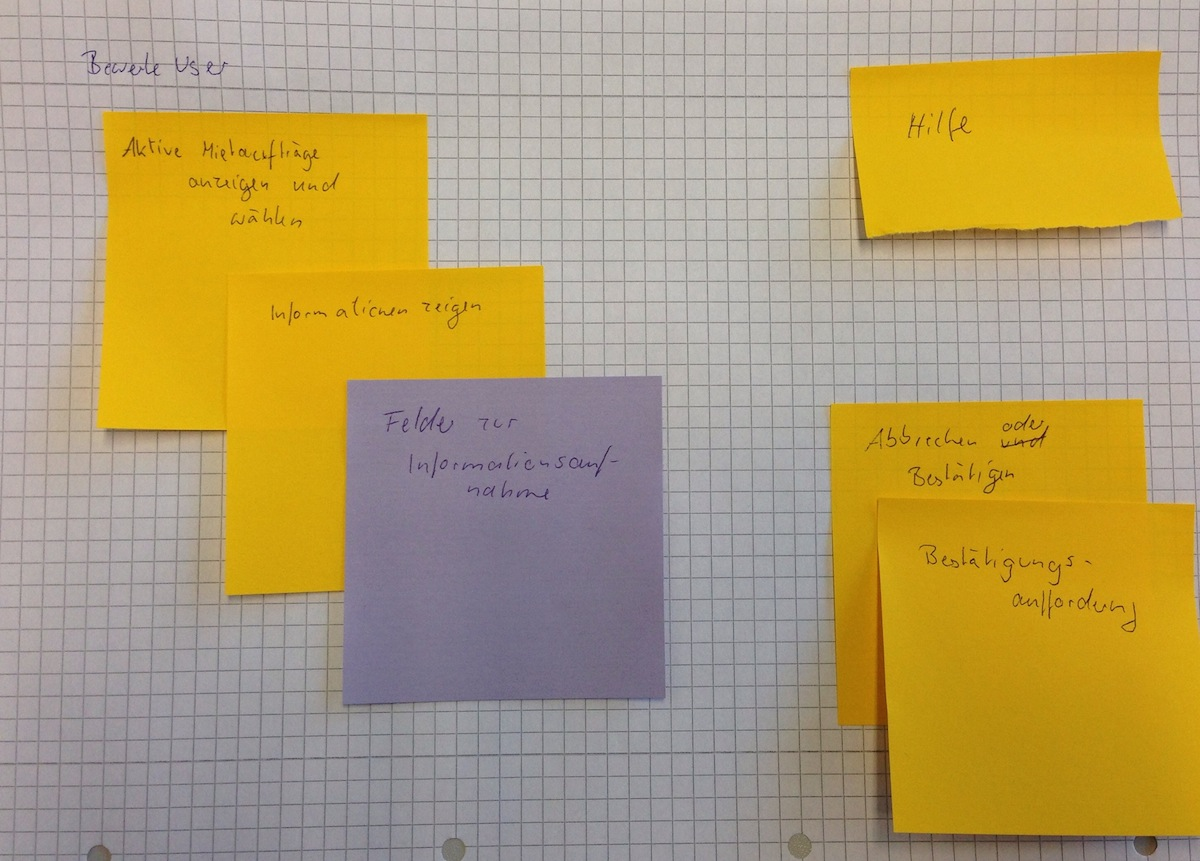
\includegraphics[width=.5\textwidth]{./images/abstract/version1/bewerteUser.JPG}}
\hfill %
\caption{Interface Con. AP1: ausloggen und bewerteUser }
\label{interfaceContents2}
\end{figure}

Beschreibung

\begin{figure}[H]
\centering
\hfill
\subfloat[bezahlungDesMietauftrags \label{pic:bezahlungDesMietauftrags}]{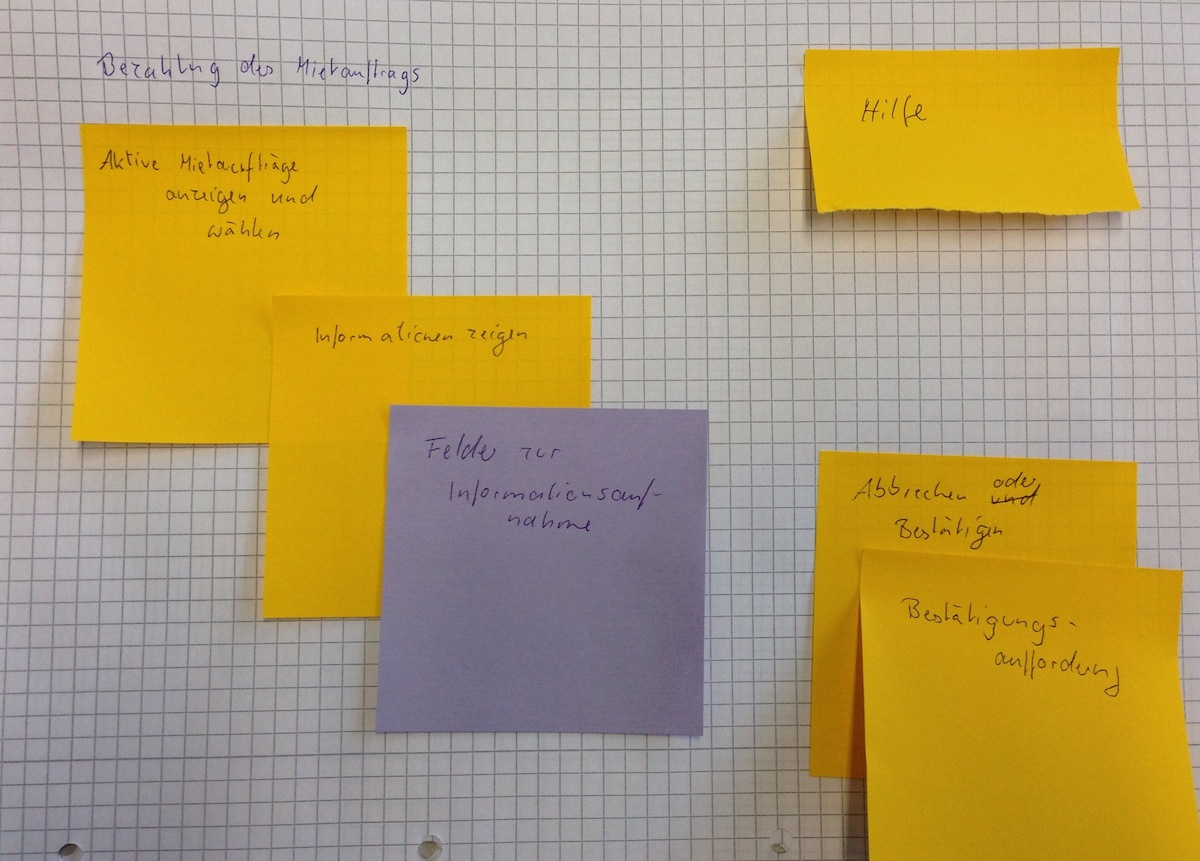
\includegraphics[width=.5\textwidth]{./images/abstract/version1/bezahlungDesMietauftrags.JPG}}
\hfill % alternativ auch \hspace{1cm} für genaue Angaben
\subfloat[kontaktiereUser \label{pic:kontaktiereUser}]{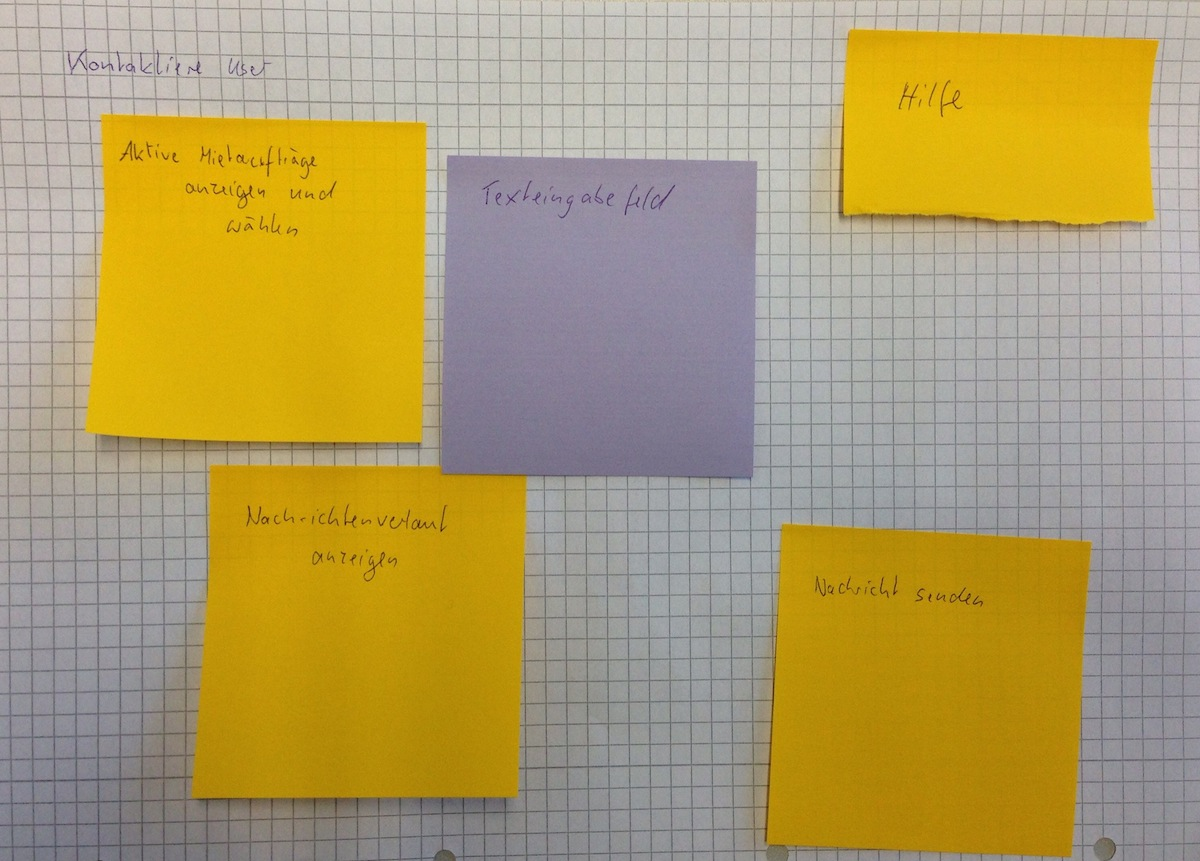
\includegraphics[width=.5\textwidth]{./images/abstract/version1/kontaktiereUser.JPG}}
\hfill %
\caption{Interface Con. AP1: bezahlungDesMietauftrags und kontaktiereUser }
\label{interfaceContents3}
\end{figure}

\begin{figure}[H]
\centering
\hfill
\subfloat[mietanfrageBeantworten \label{pic:mietanfrageBeantworten}]{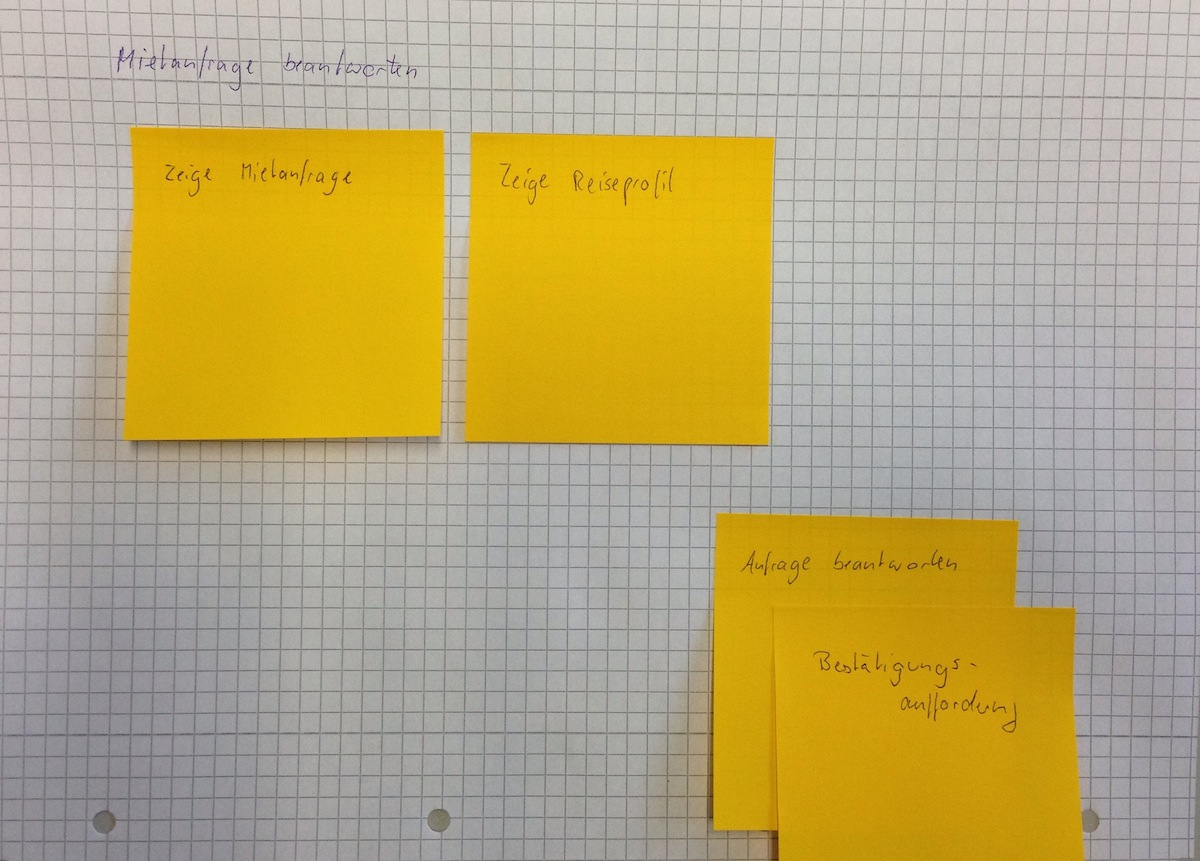
\includegraphics[width=.5\textwidth]{./images/abstract/version1/mietanfrageBeantworten.JPG}}
\hfill % alternativ auch \hspace{1cm} für genaue Angaben
\subfloat[profilVerwalten \label{pic:profilVerwalten}]{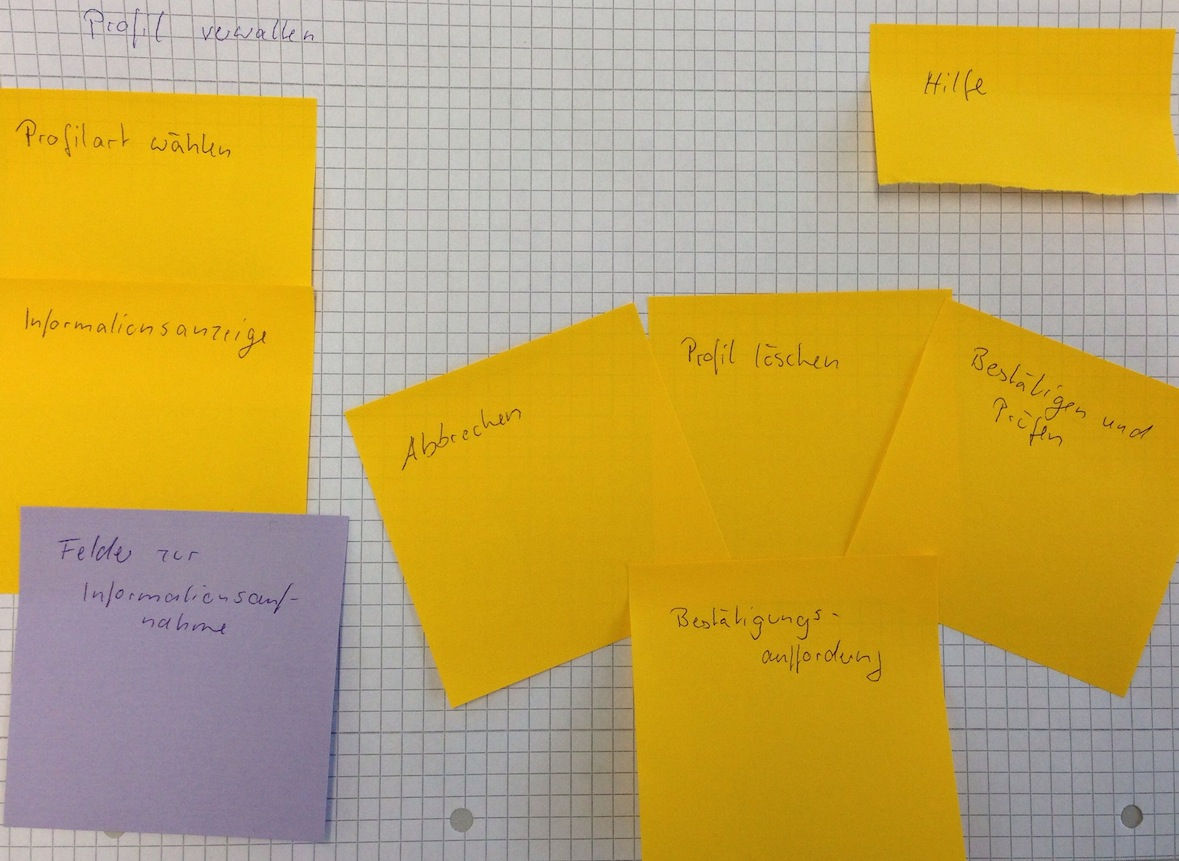
\includegraphics[width=.5\textwidth]{./images/abstract/version1/profilVerwalten.JPG}}
\hfill %
\caption{Interface Con. AP1: mietanfrageBeantworten und profilVerwalten }
\label{interfaceContents4}
\end{figure}

Beschreibung

\begin{figure}[H]
\centering
\hfill
\subfloat[registrierung \label{pic:registrierung}]{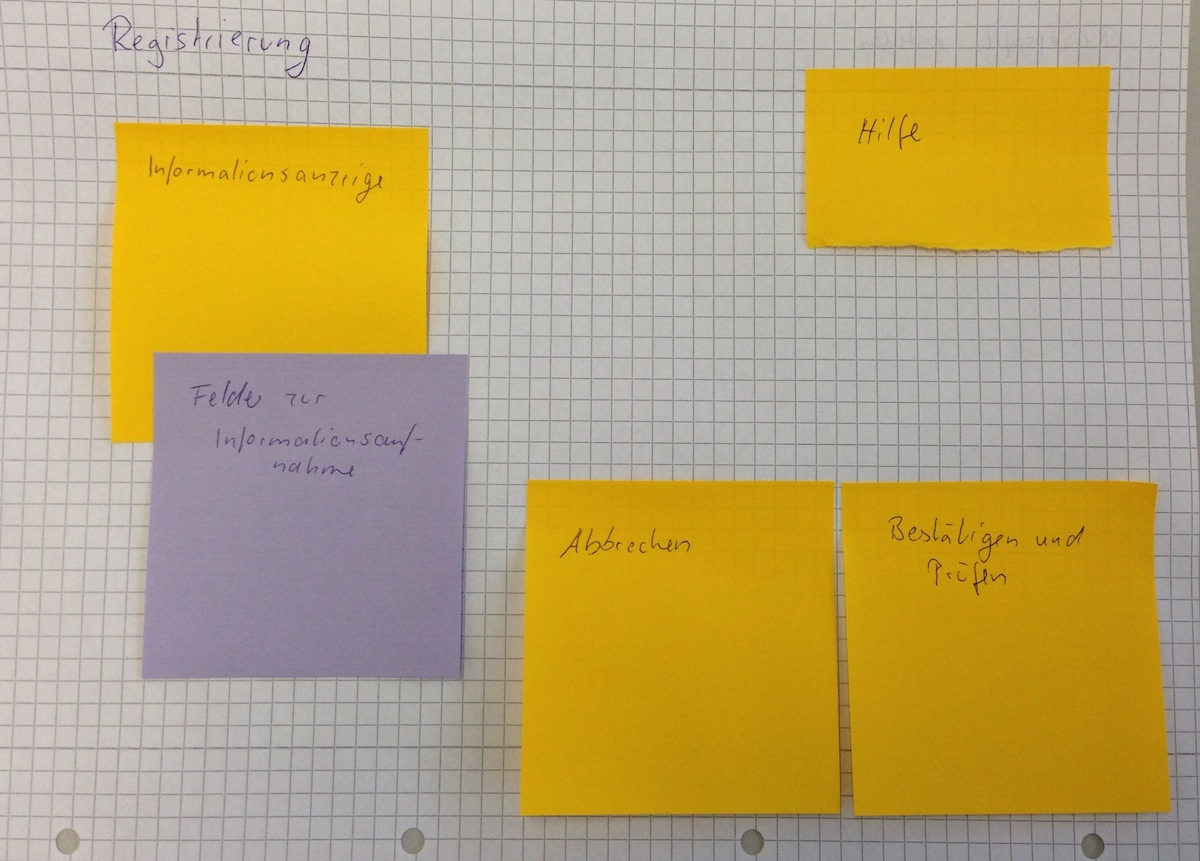
\includegraphics[width=.5\textwidth]{./images/abstract/version1/registrierung.JPG}}
\hfill % alternativ auch \hspace{1cm} für genaue Angaben
\subfloat[reiseprofilErstellen \label{pic:reiseprofilErstellen}]{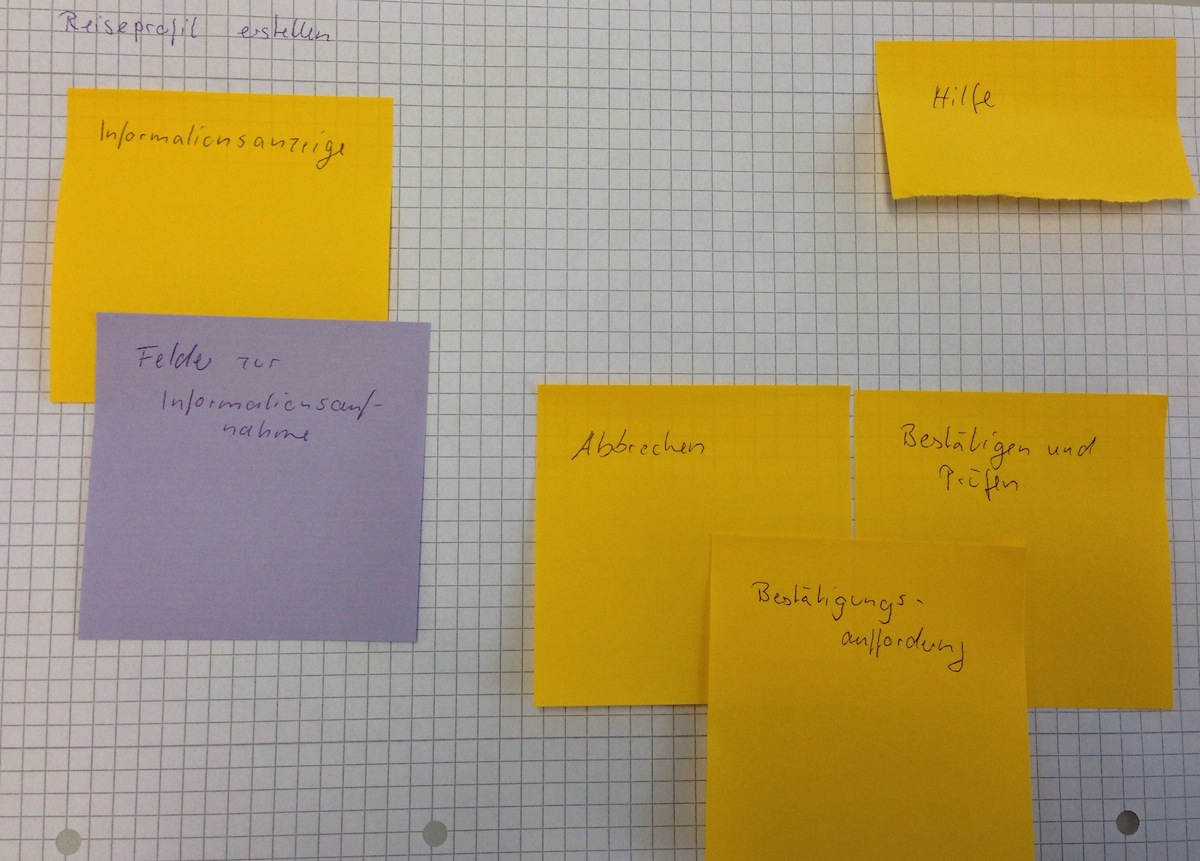
\includegraphics[width=.5\textwidth]{./images/abstract/version1/reiseprofilErstellen.JPG}}
\hfill %
\caption{Interface Con. AP1: registrierung und reiseprofilErstellen }
\label{interfaceContents5}
\end{figure}

\begin{figure}[H]
\centering
\hfill
\subfloat[rueckmeldung \label{pic:rueckmeldung}]{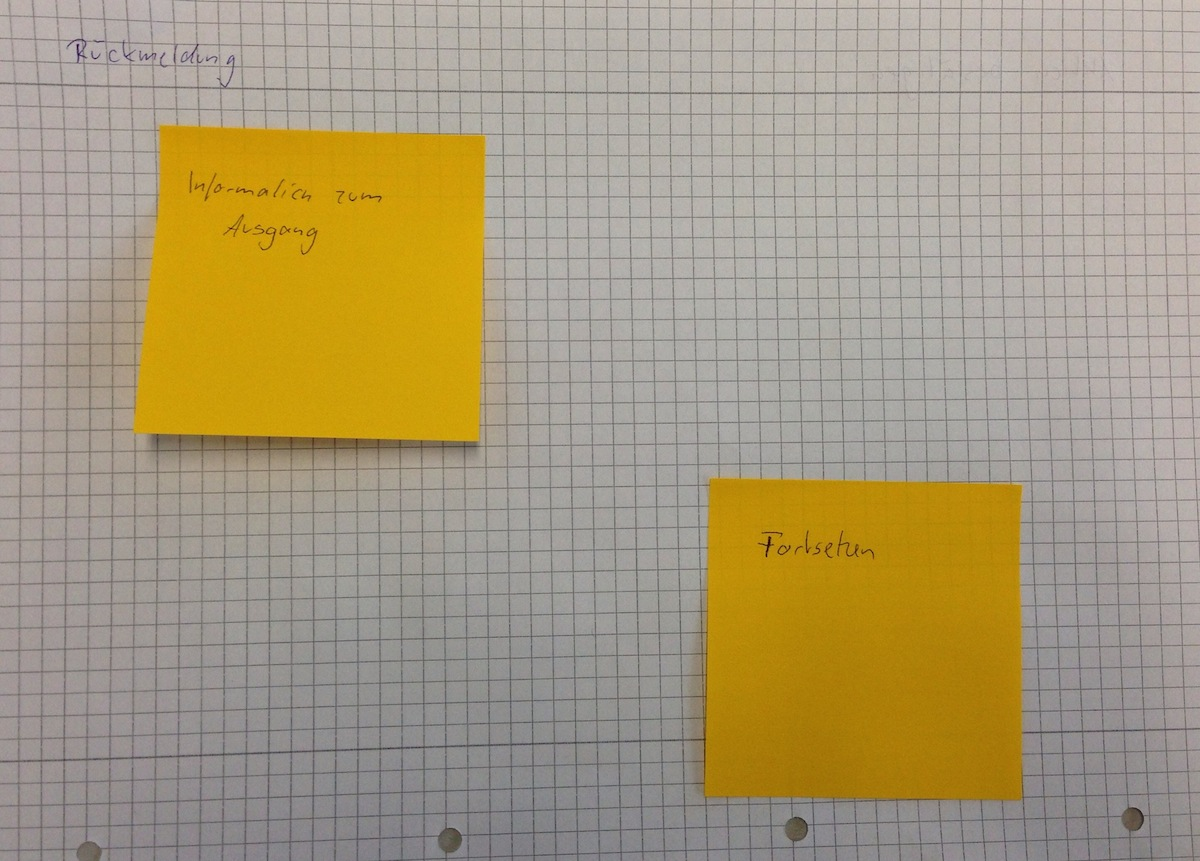
\includegraphics[width=.5\textwidth]{./images/abstract/version1/rueckmeldung.JPG}}
\hfill % alternativ auch \hspace{1cm} für genaue Angaben
\subfloat[sucheMietobjekt \label{pic:sucheMietobjekt}]{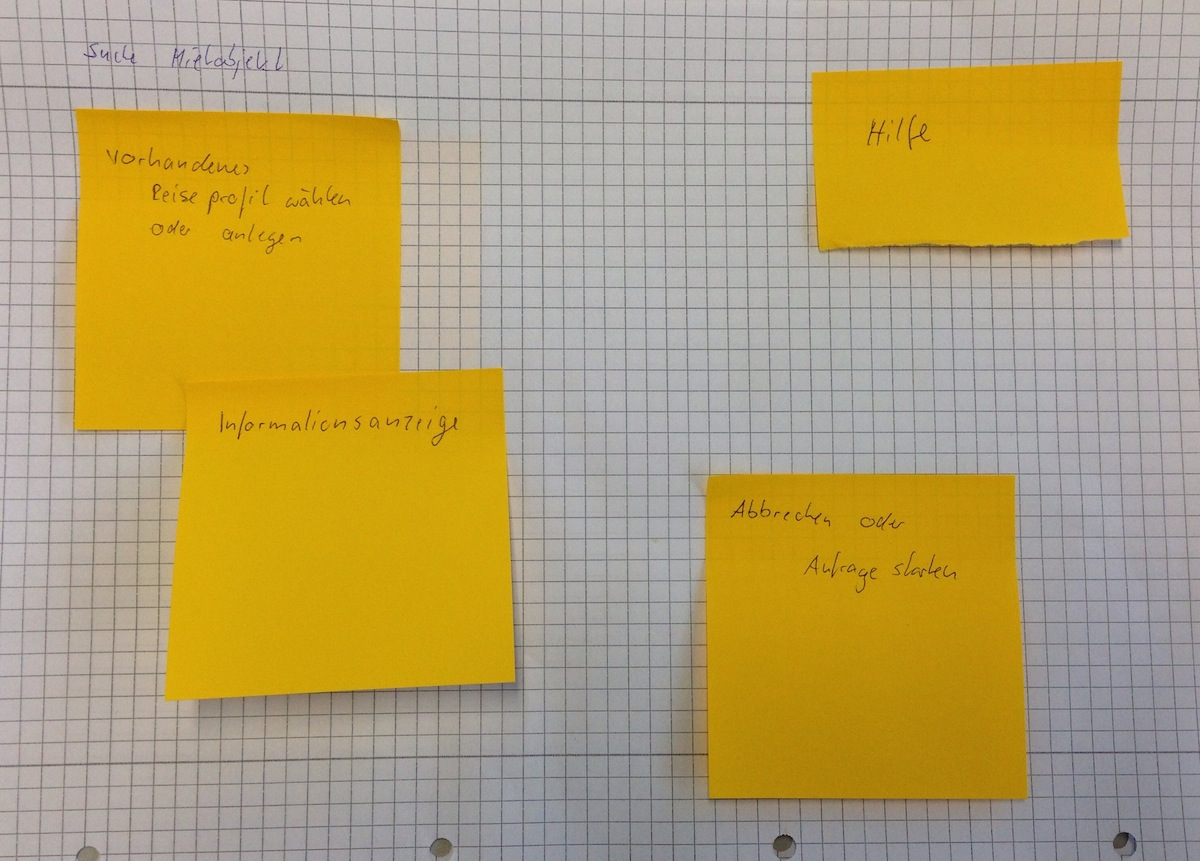
\includegraphics[width=.5\textwidth]{./images/abstract/version1/sucheMietobjekt.JPG}}
\hfill %
\caption{Interface Con. AP1: rueckmeldung und sucheMietobjekt }
\label{interfaceContents6}
\end{figure}

Beschreibung

\begin{figure}[H]
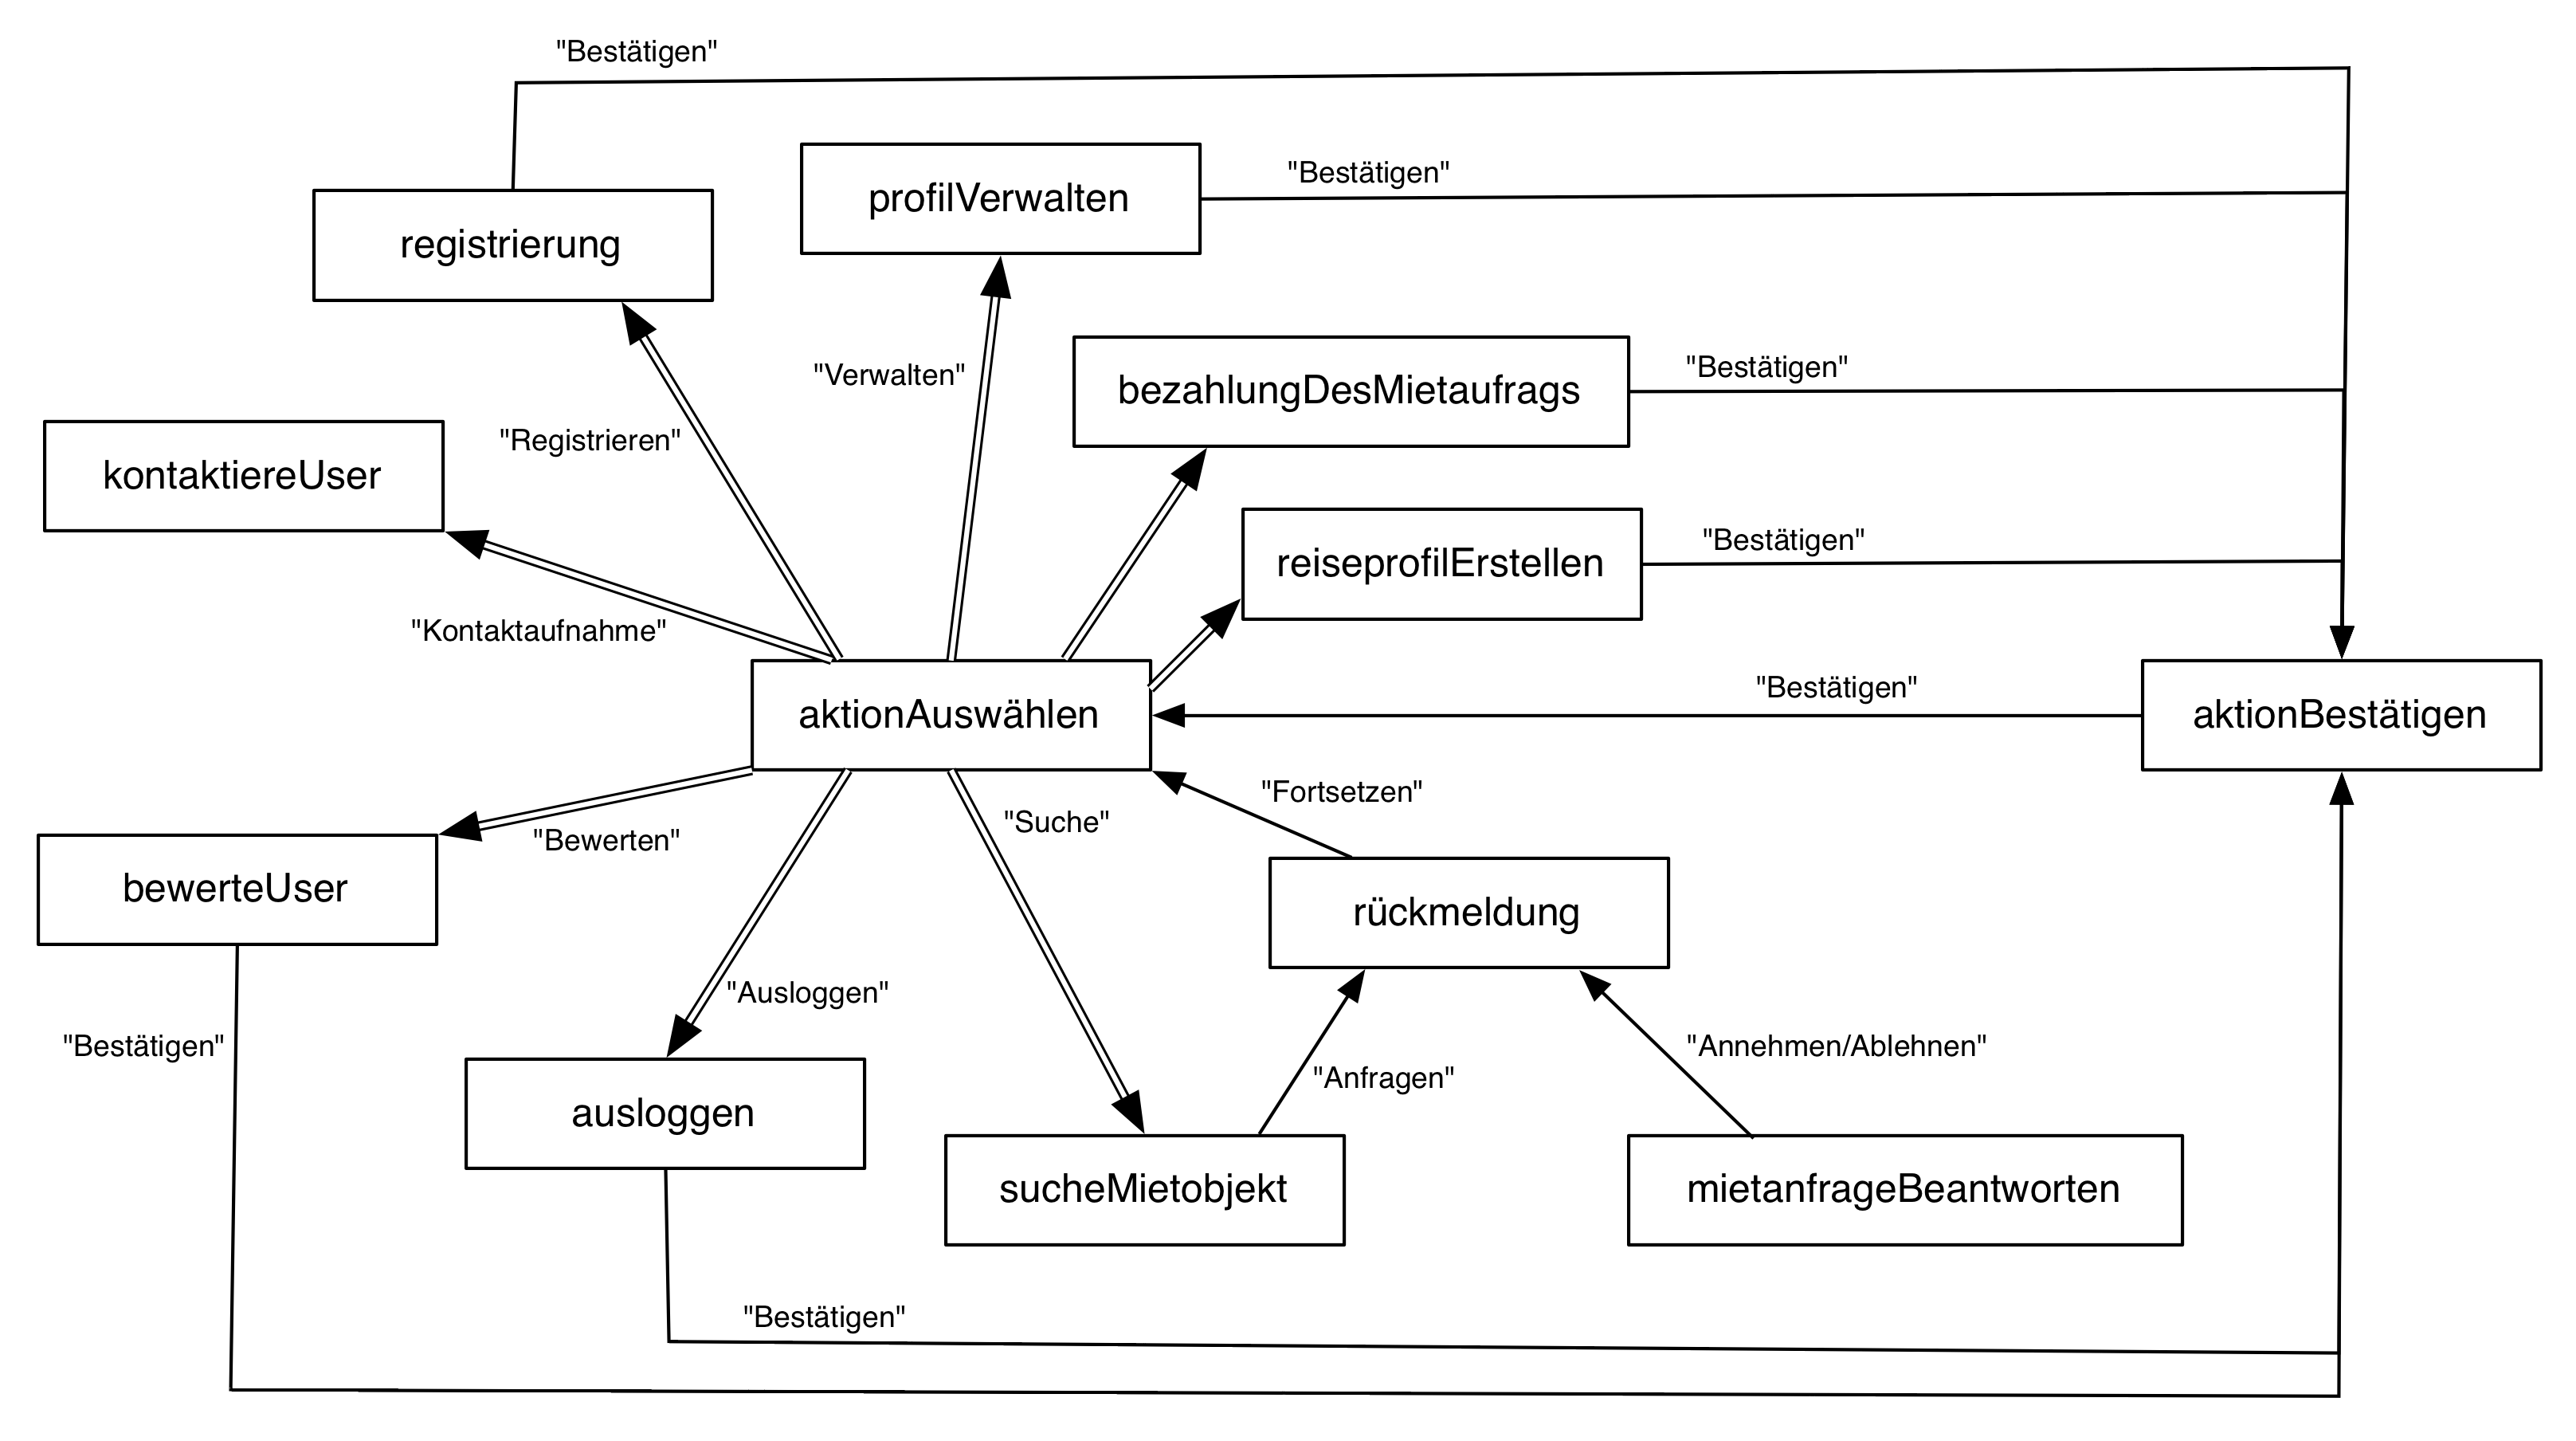
\includegraphics[width=1\textwidth]{./images/navigationmap1.png}
\caption{Context Navigation Map Version 1}
\label{fig:navigationmap1}
\end{figure}


\newpage

\subsection{Abstract Prototype 2}

\begin{figure}[H]
\centering
\hfill
\subfloat[anmelden \label{pic:anmelden}]{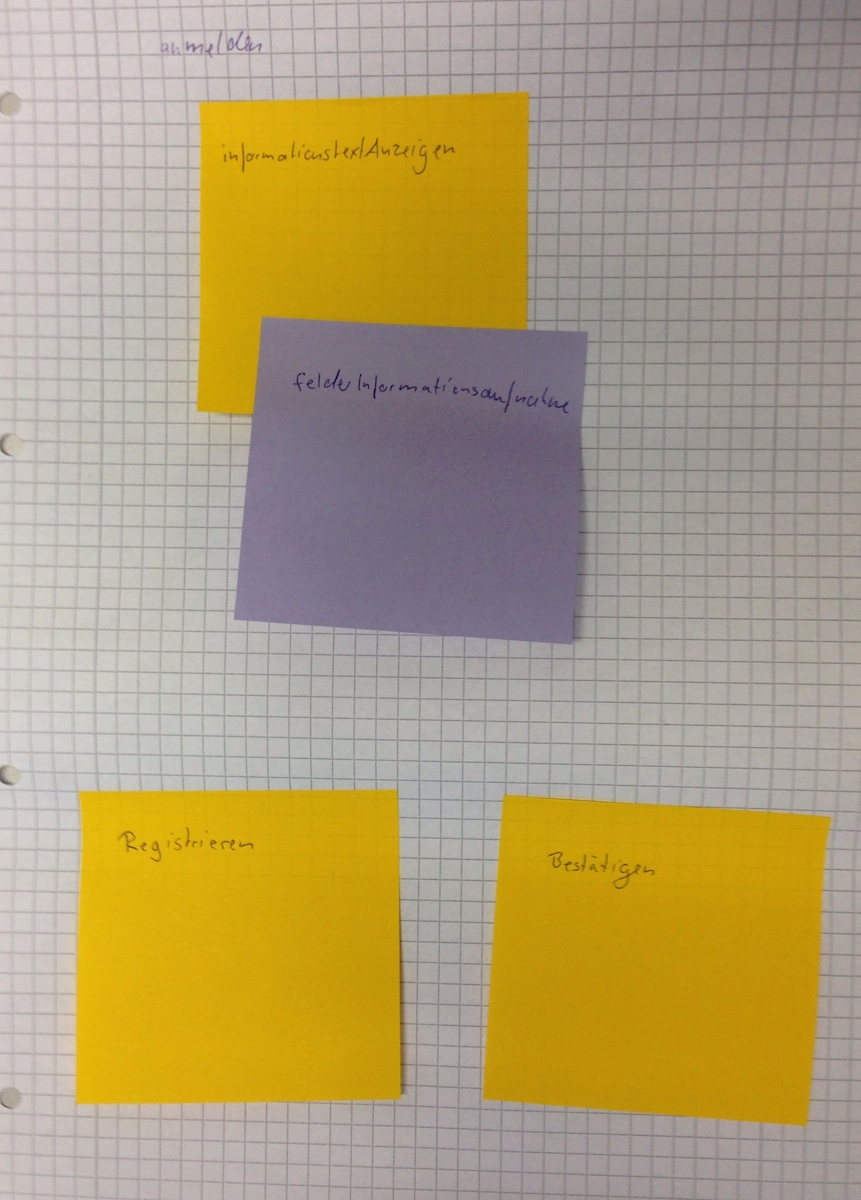
\includegraphics[width=.5\textwidth]{./images/abstract/version2/anmelden.JPG}}
\hfill % alternativ auch \hspace{1cm} für genaue Angaben
\subfloat[neuenBenutzerRegistrieren \label{pic:neuenBenutzerRegistrieren}]{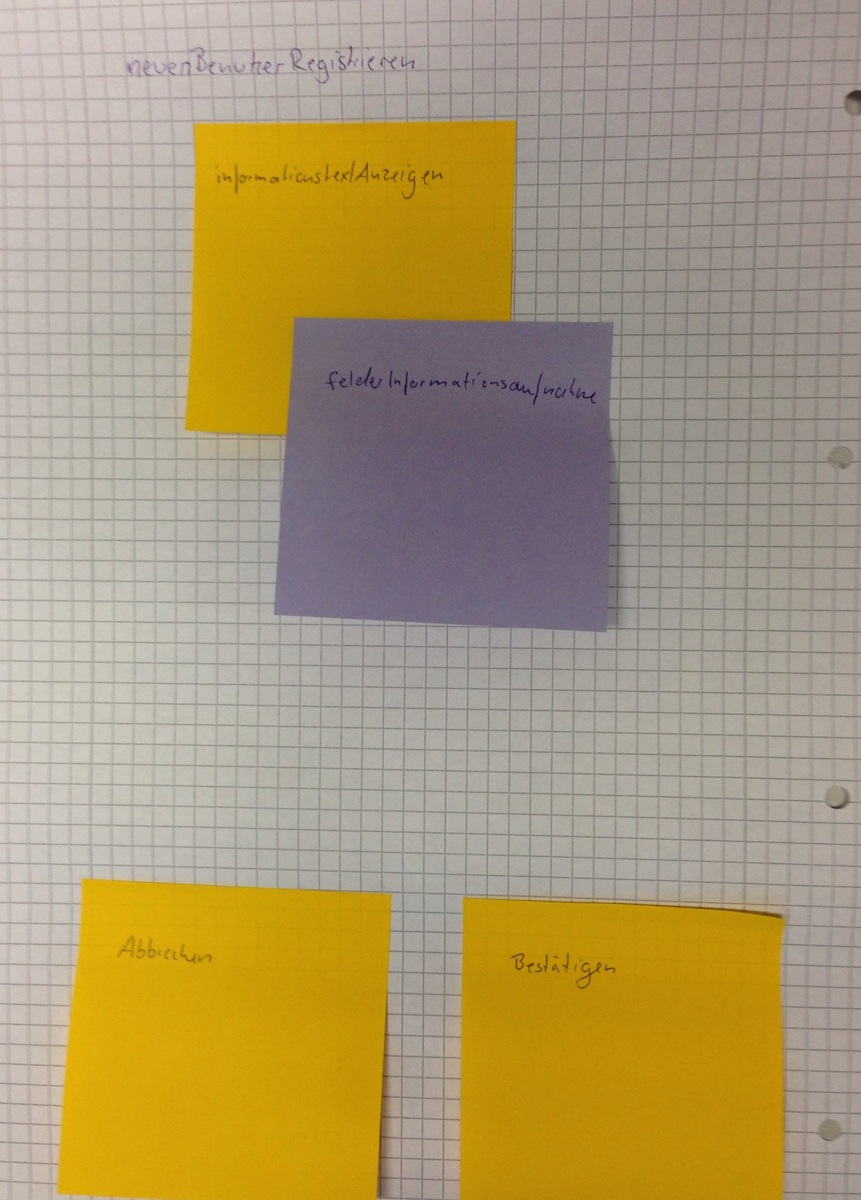
\includegraphics[width=.5\textwidth]{./images/abstract/version2/neuenBenutzerRegistrieren.JPG}}
\hfill %
\caption{Interface Con. AP2: anmelden und neuenBenutzerRegistrieren }
\label{interfaceContents7}
\end{figure}

Beschreibung

\begin{figure}[H]
\centering
\hfill
\subfloat[anzeigenVorhandenerAktionen \label{pic:anzeigenVorhandenerAktionen}]{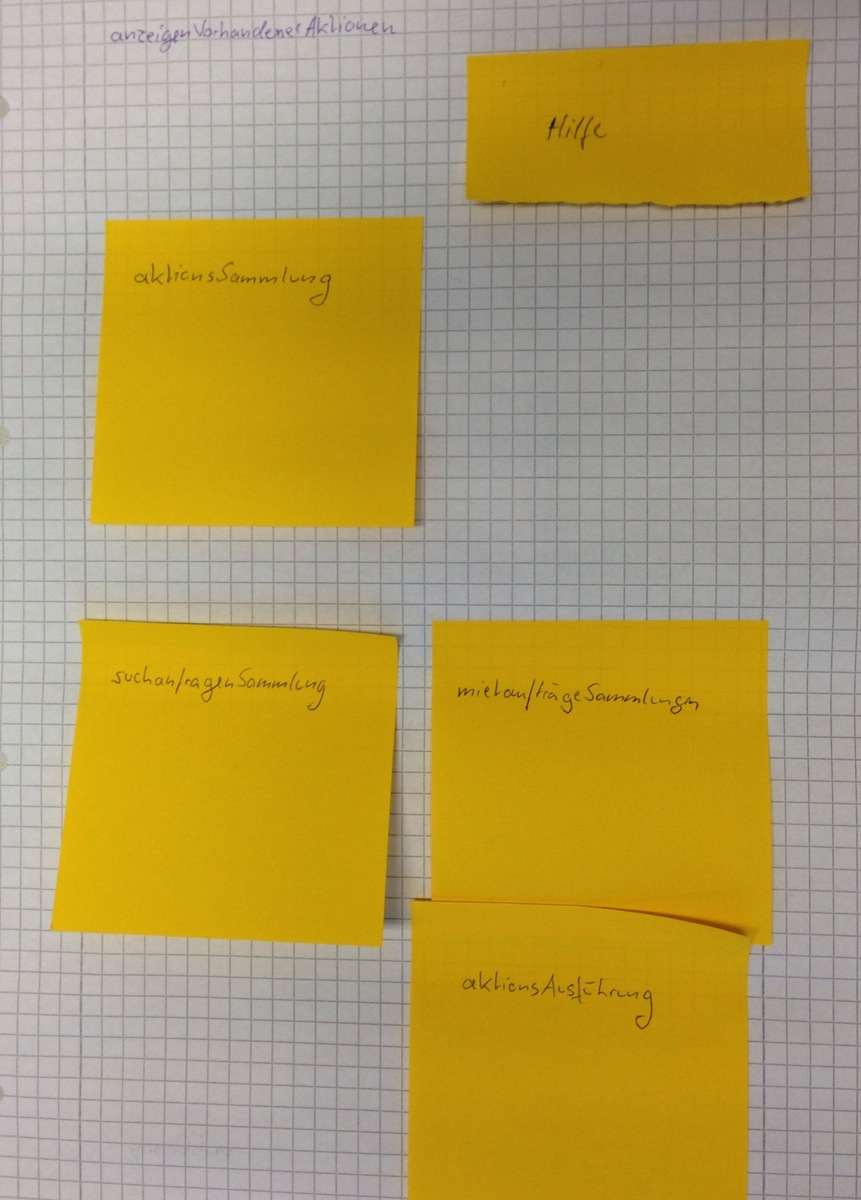
\includegraphics[width=.5\textwidth]{./images/abstract/version2/anzeigenVorhandenerAktionen.JPG}}
\hfill % alternativ auch \hspace{1cm} für genaue Angaben
\subfloat[anzeigeDerSuchanfrage \label{pic:anzeigeDerSuchanfrage}]{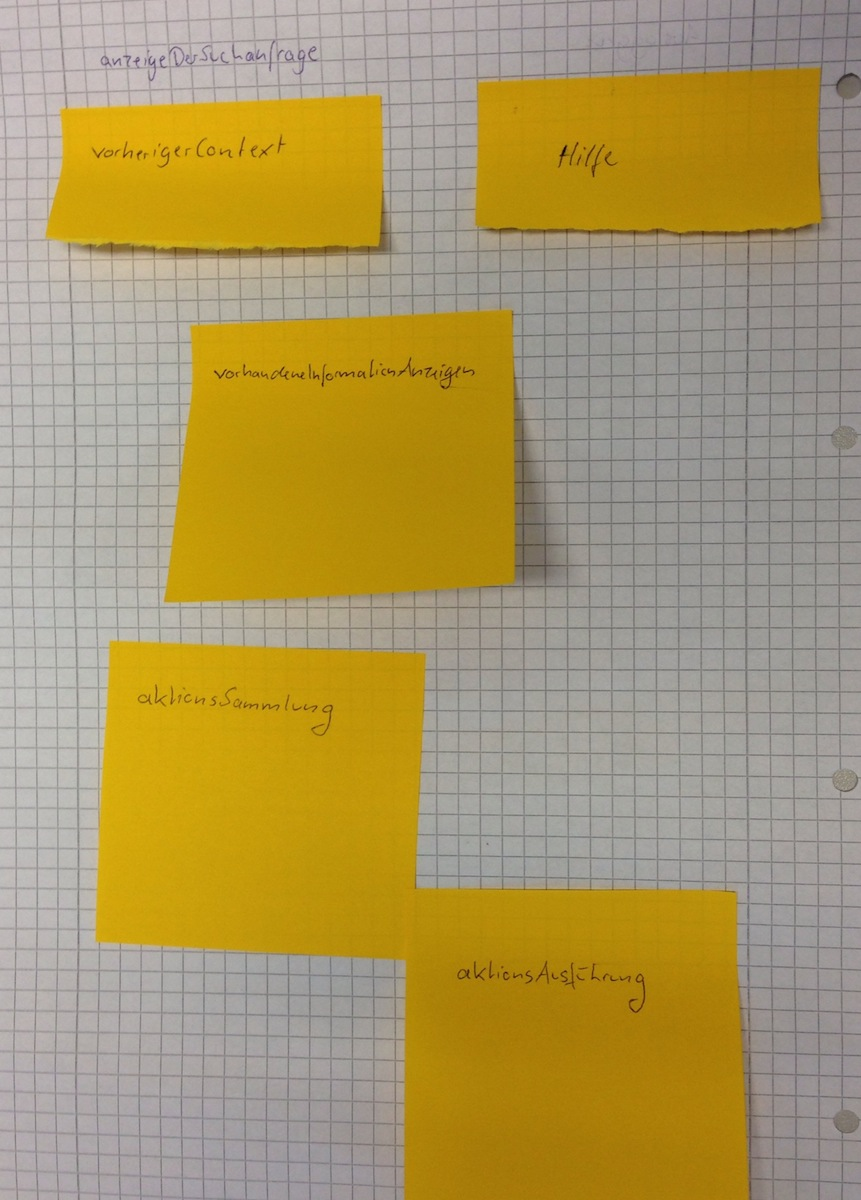
\includegraphics[width=.5\textwidth]{./images/abstract/version2/anzeigeDerSuchanfrage.JPG}}
\hfill %
\caption{Interface Con. AP2: anzeigenVorhandenerAktionen und anzeigeDerSuchanfrage }
\label{interfaceContents8}
\end{figure}

Beschreibung

\begin{figure}[H]
\centering
\hfill
\subfloat[benutzerprofilVerwalten \label{pic:benutzerprofilVerwalten}]{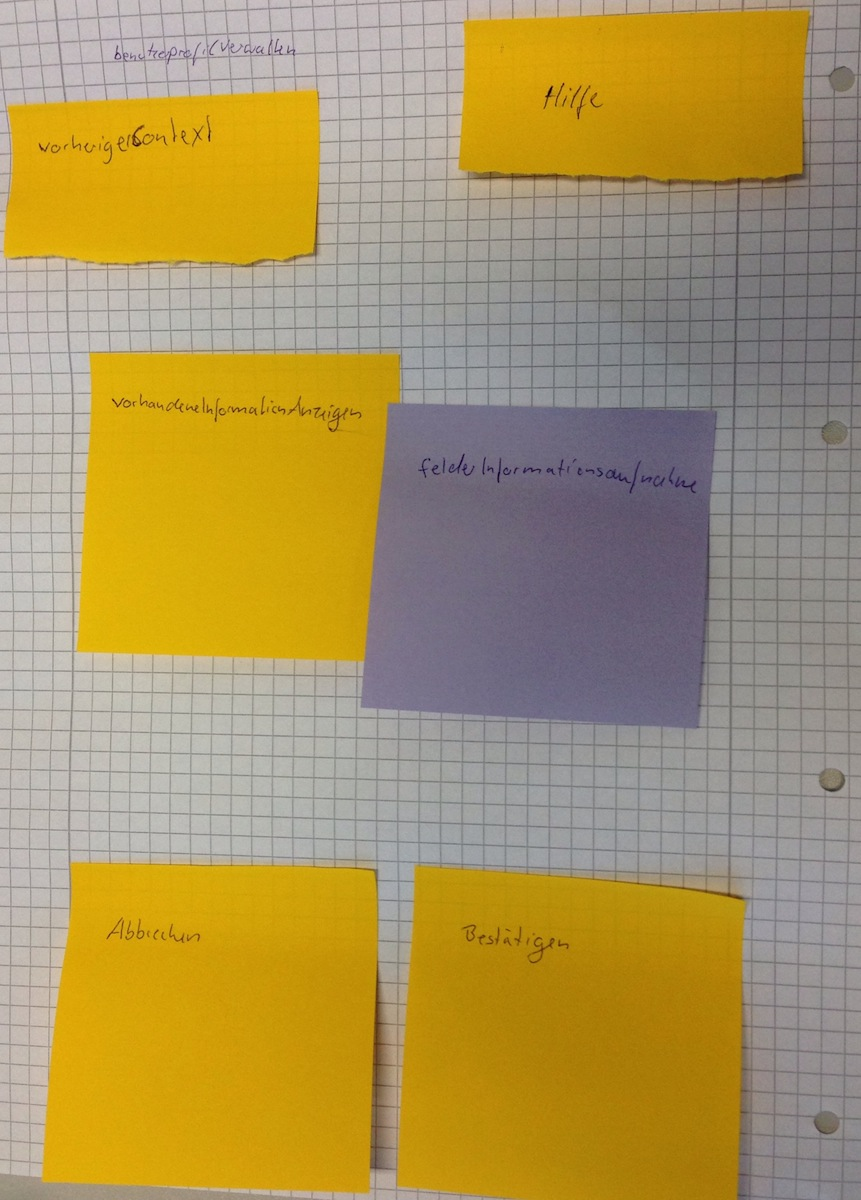
\includegraphics[width=.5\textwidth]{./images/abstract/version2/benutzerprofilVerwalten.JPG}}
\hfill % alternativ auch \hspace{1cm} für genaue Angaben
\subfloat[bestätigung \label{pic:bestaetigung}]{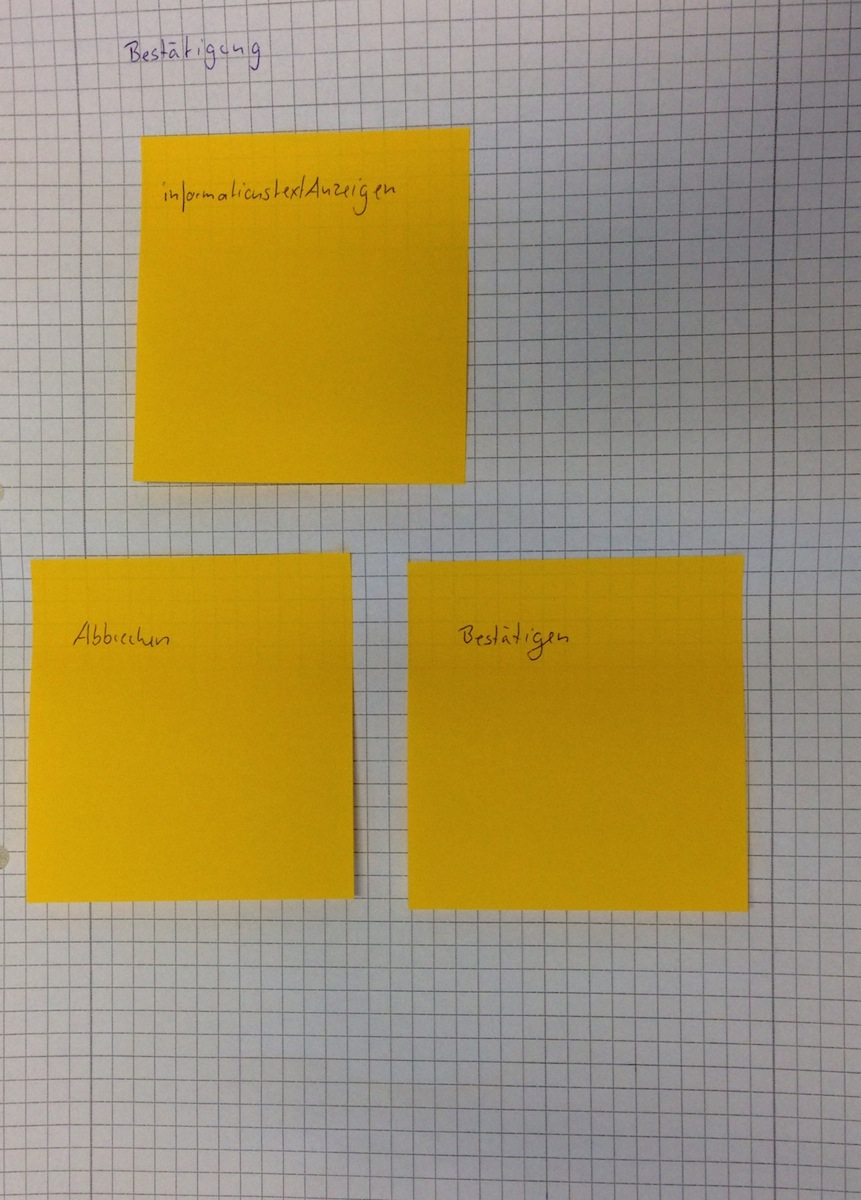
\includegraphics[width=.5\textwidth]{./images/abstract/version2/bestaetigung.JPG}}
\hfill %
\caption{Interface Con. AP2: benutzerprofilVerwalten und bestätigung }
\label{interfaceContents9}
\end{figure}

Beschreibung

\begin{figure}[H]
\centering
\hfill
\subfloat[kontaktaufnahme \label{pic:kontaktaufnahme}]{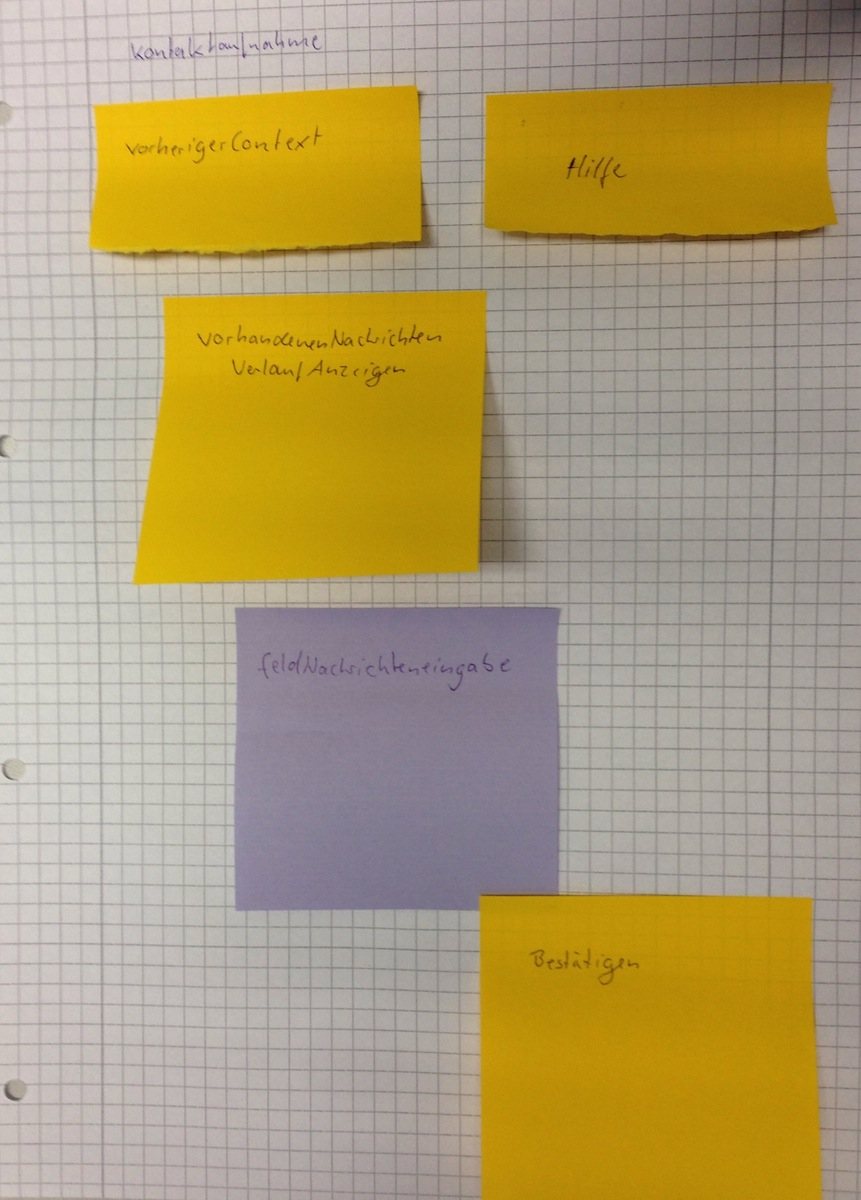
\includegraphics[width=.5\textwidth]{./images/abstract/version2/kontaktaufnahme.JPG}}
\hfill % alternativ auch \hspace{1cm} für genaue Angaben
\subfloat[mietanfragenAnzeigen \label{pic:mietanfragenAnzeigen}]{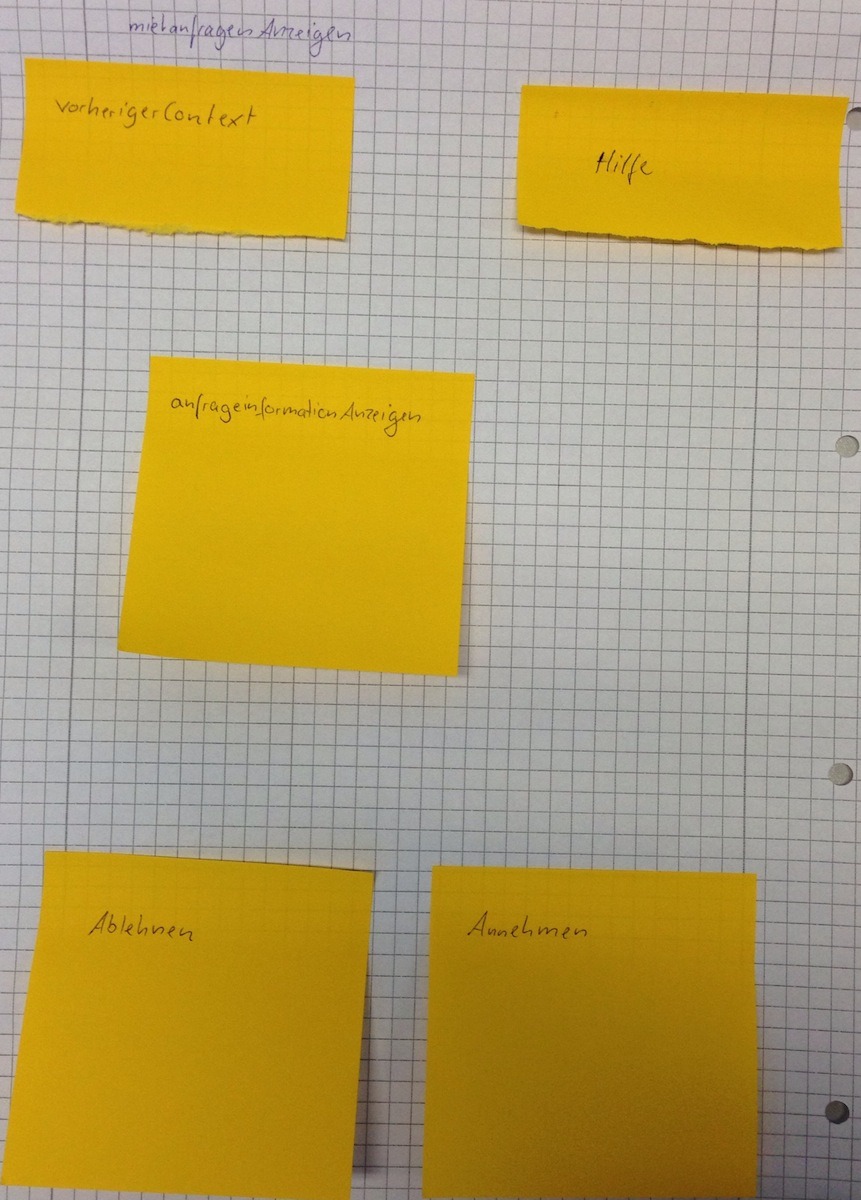
\includegraphics[width=.5\textwidth]{./images/abstract/version2/mietanfragenAnzeigen.JPG}}
\hfill %
\caption{Interface Con. AP2: kontaktaufnahme und mietanfragenAnzeigen }
\label{interfaceContents10}
\end{figure}

Beschreibung

\begin{figure}[H]
\centering
\hfill
\subfloat[mietobjekteVerwalten \label{pic:mietobjekteVerwalten}]{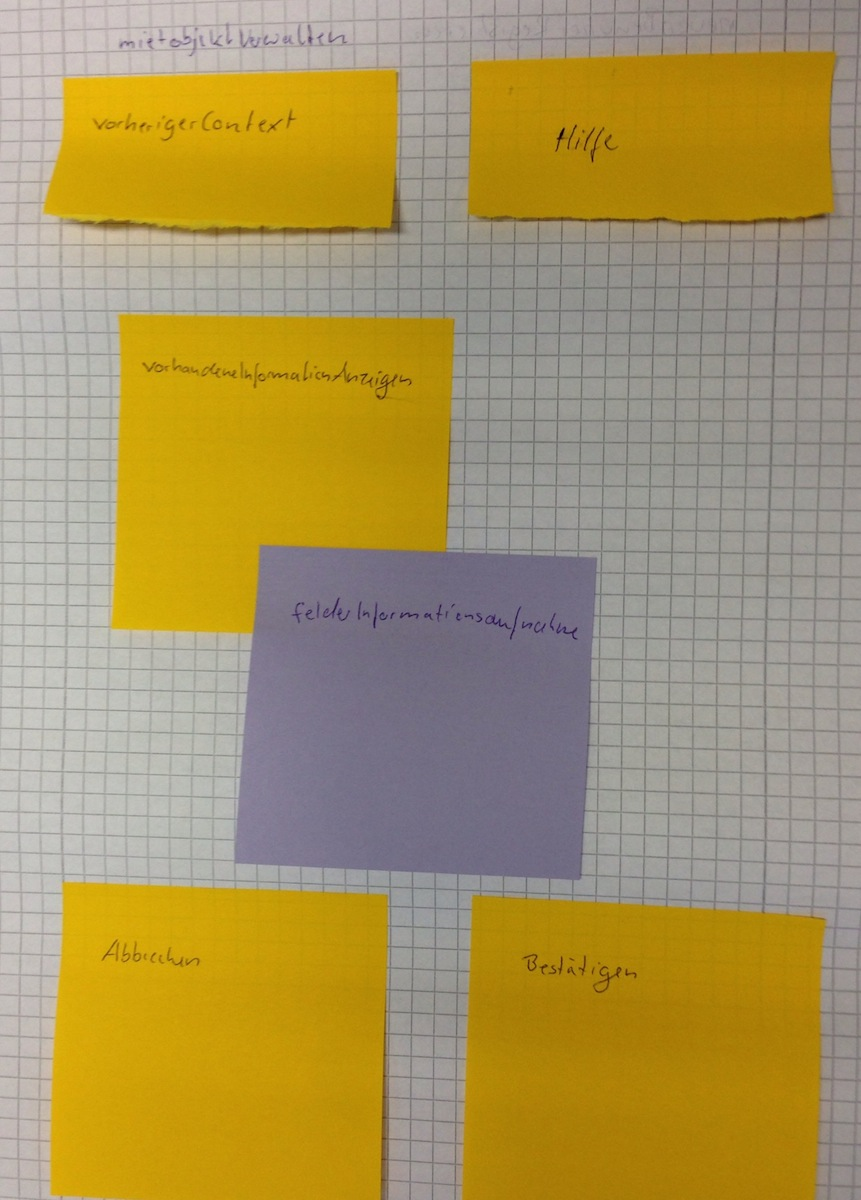
\includegraphics[width=.5\textwidth]{./images/abstract/version2/mietobjekteVerwalten.JPG}}
\hfill % alternativ auch \hspace{1cm} für genaue Angaben
\subfloat[suchanfrageStarten \label{pic:suchanfrageStarten}]{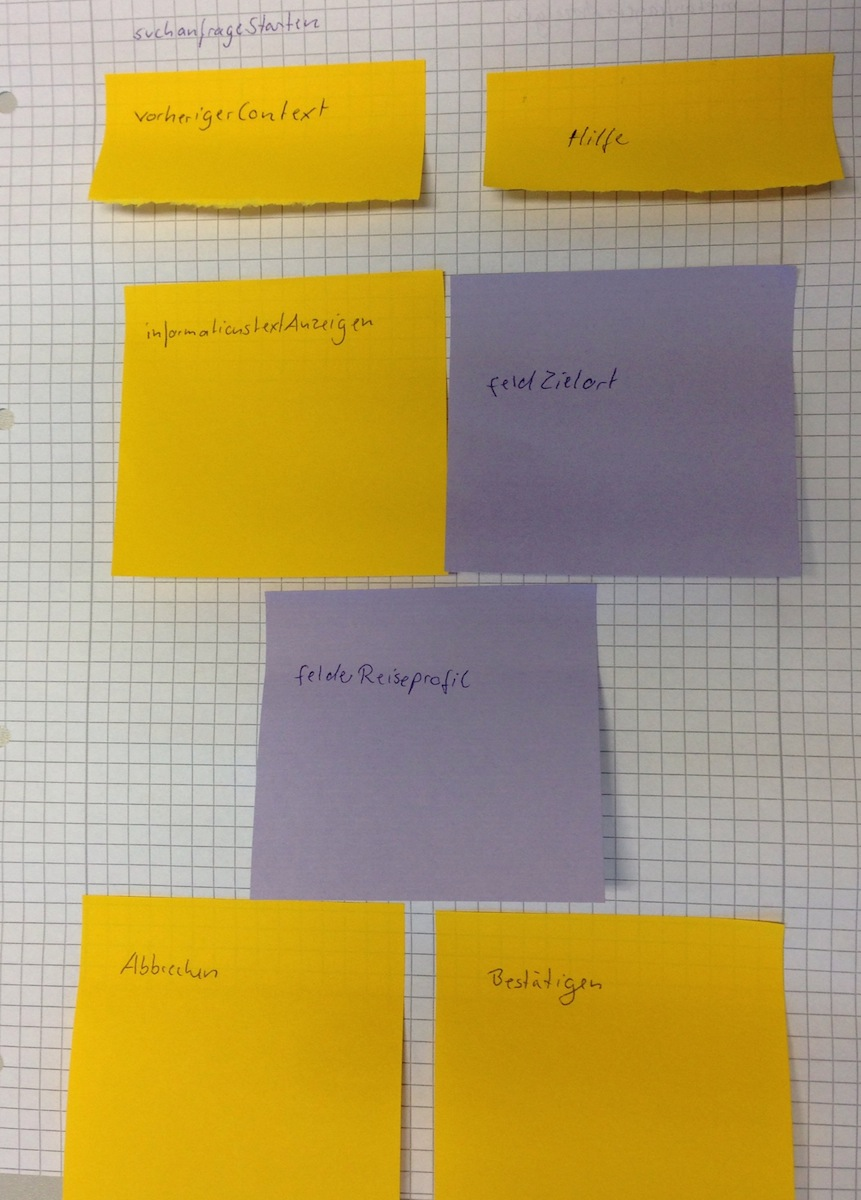
\includegraphics[width=.5\textwidth]{./images/abstract/version2/suchanfragenStarten.JPG}}
\hfill %
\caption{Interface Con. AP2: mietobjekteVerwalten und suchanfrageStarten }
\label{interfaceContents11}
\end{figure}

Beschreibung

\begin{figure}[H]
\centering
\hfill
\subfloat[userBewertung \label{pic:userBewertung}]{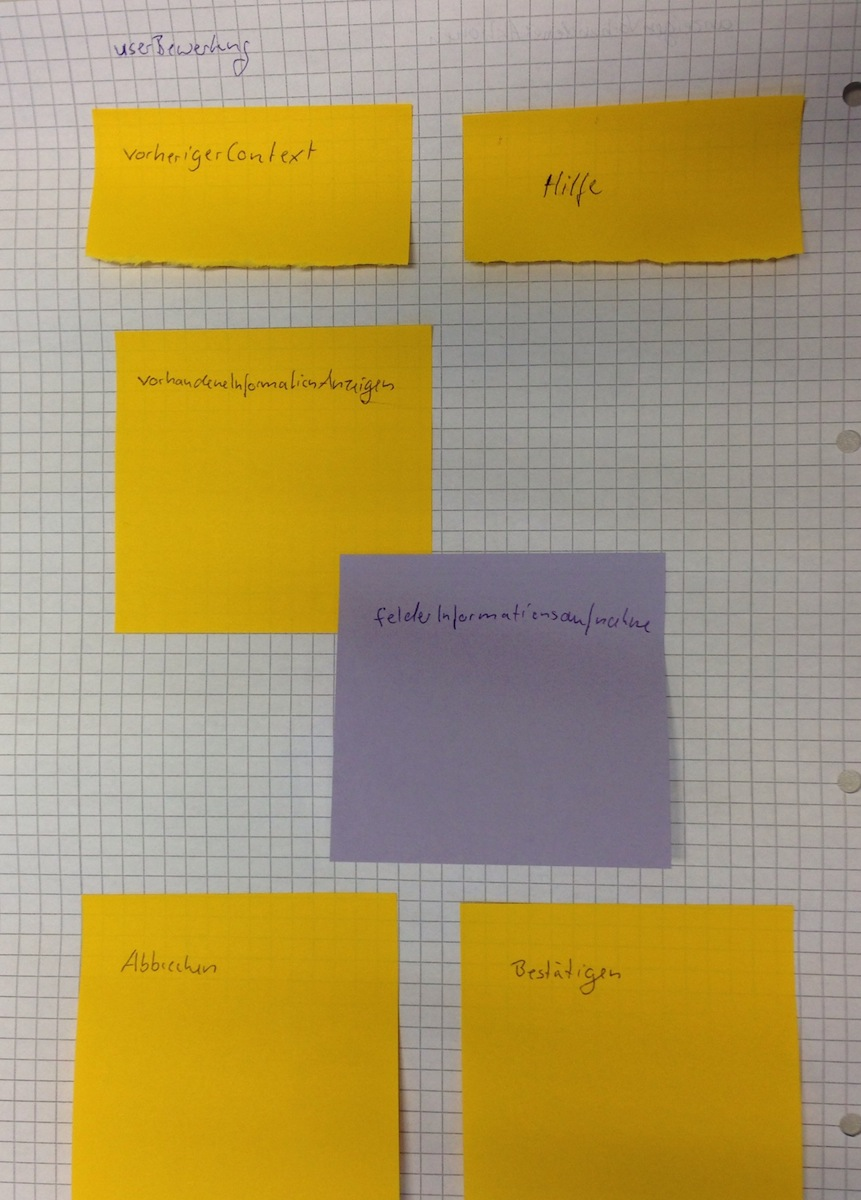
\includegraphics[width=.5\textwidth]{./images/abstract/version2/userBewertung.JPG}}
\hfill % alternativ auch \hspace{1cm} für genaue Angaben
\subfloat[vorhandeneMietobjekteAnzeigen \label{pic:vorhandeneMietobjekteAnzeigen}]{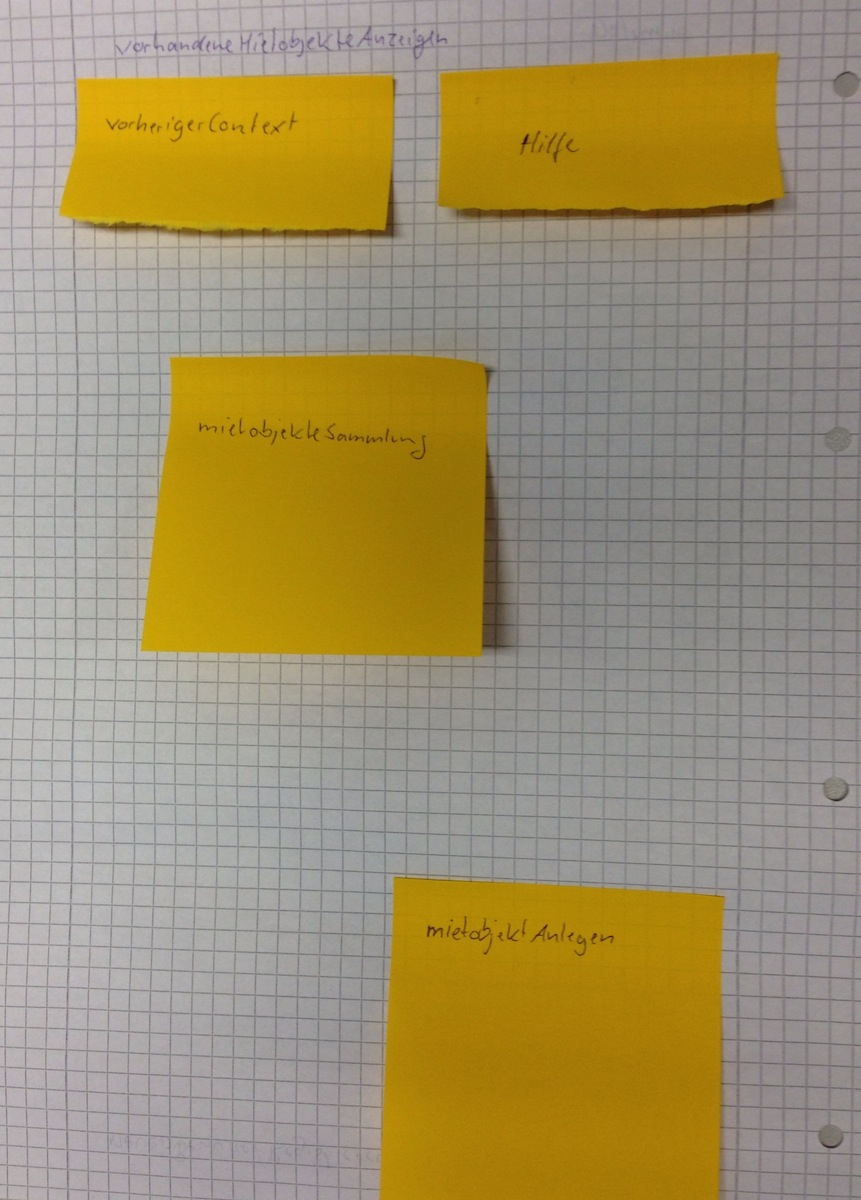
\includegraphics[width=.5\textwidth]{./images/abstract/version2/vorhandeneMietobjekteAnzeigen.JPG}}
\hfill %
\caption{Interface Con. AP2: userBewertung und vorhandeneMietobjekteAnzeigen }
\label{interfaceContents12}
\end{figure}

Beschreibung

\begin{wrapfigure}{r}{0cm}
\centering
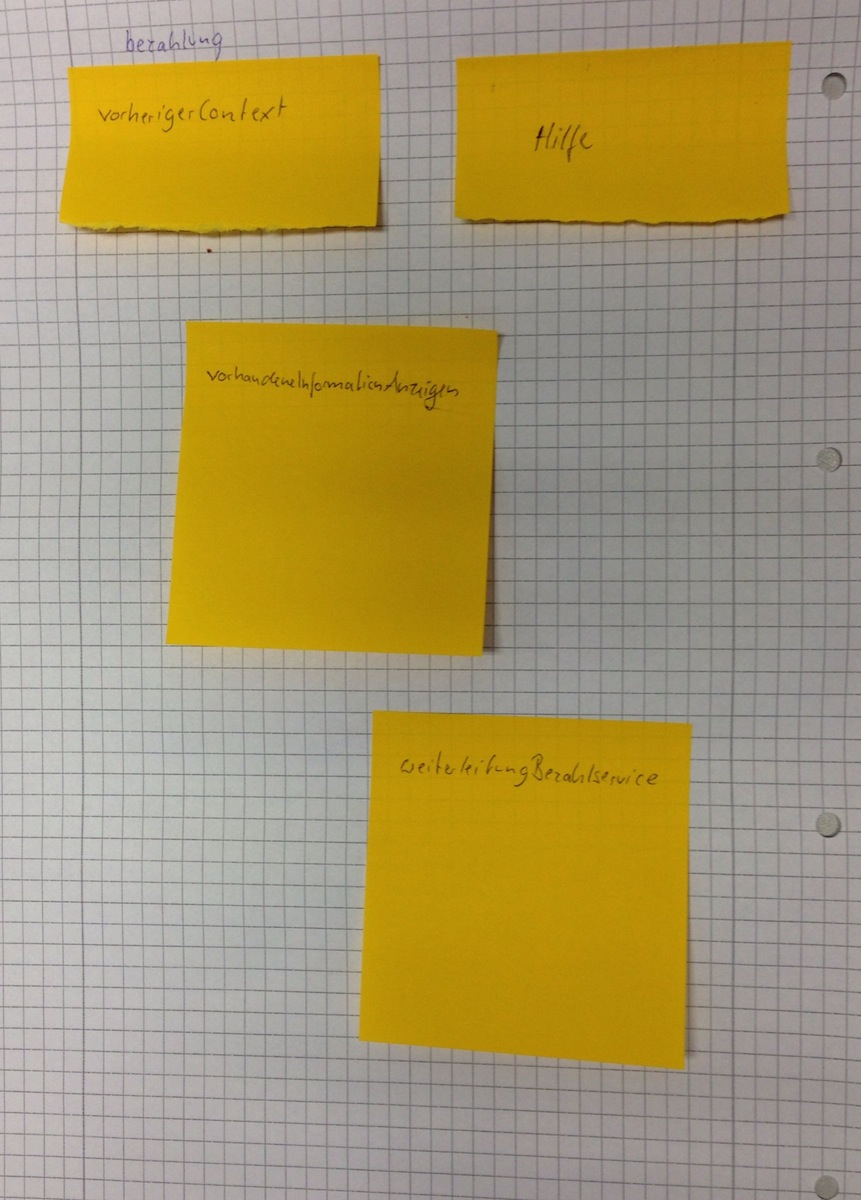
\includegraphics[width=.5\textwidth]{./images/abstract/version2/bezahlung.JPG}
\caption{Int. Con. AP2: bezahlung}
\label{interfaceContents13}
\end{wrapfigure}


testestsetset

\begin{figure}[H]
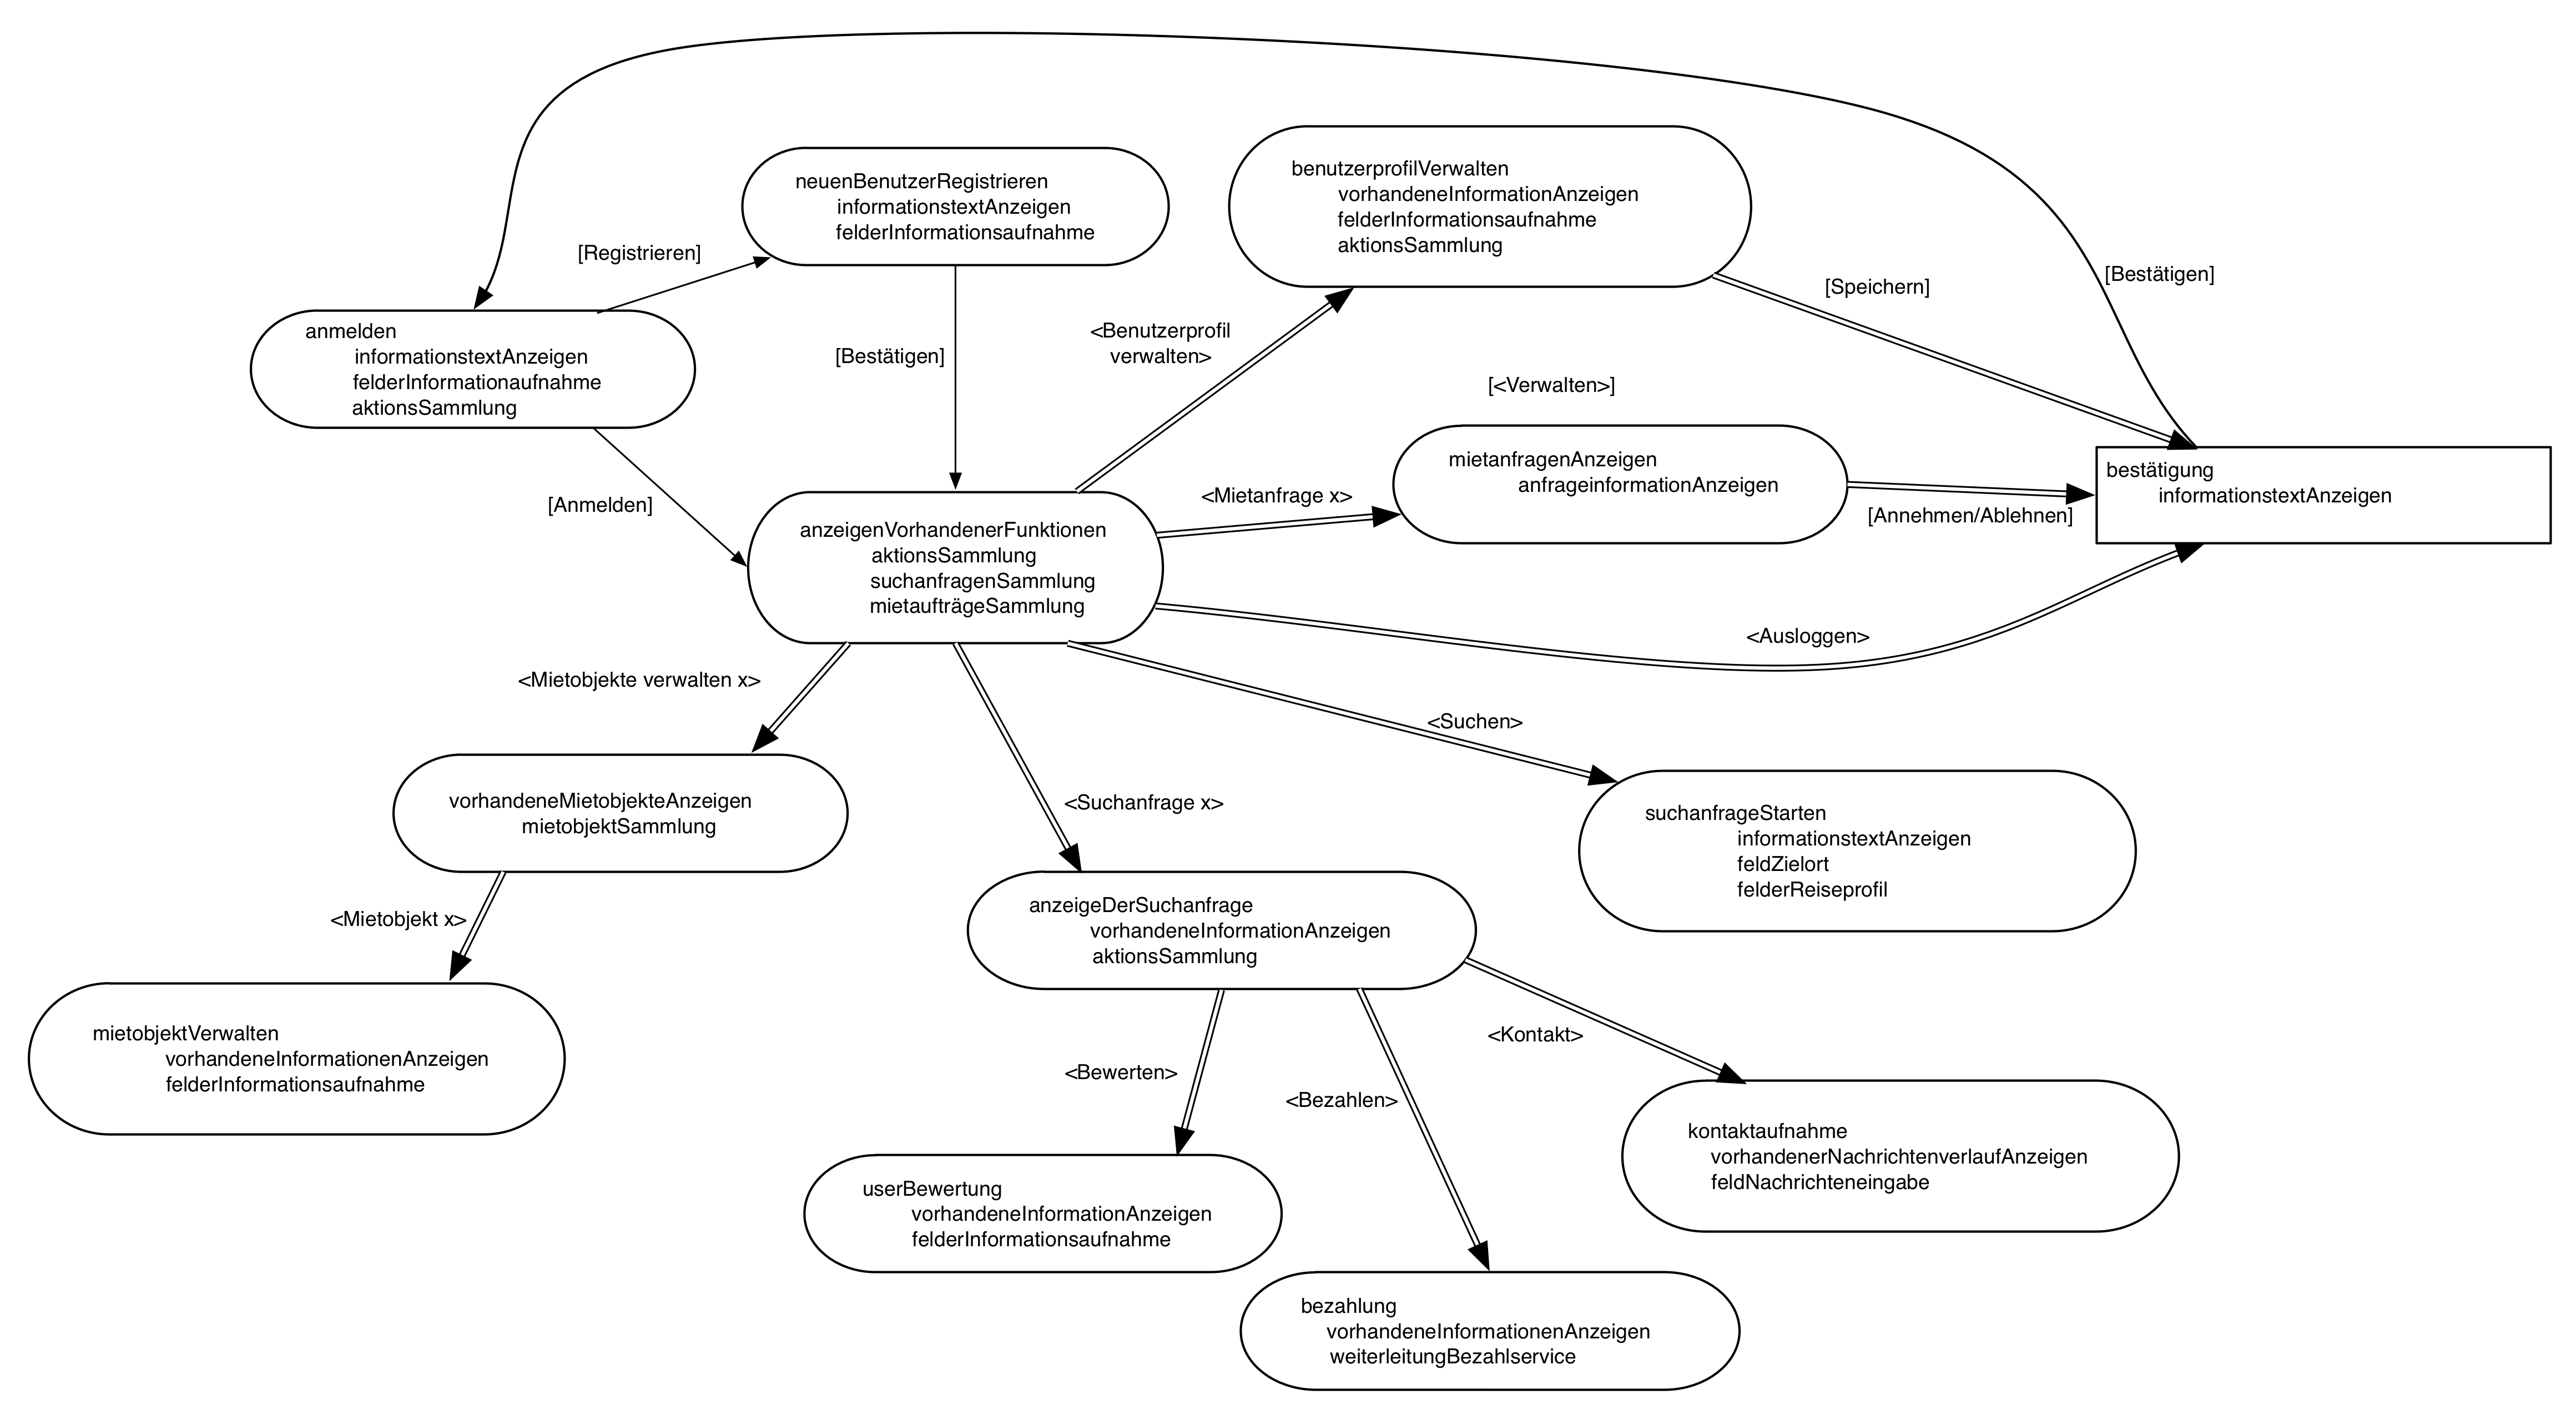
\includegraphics[width=1\textwidth]{./images/navigationmap2.png}
\caption{Context Navigation Map Version 2}
\label{fig:navigationmap2}
\end{figure}


\newpage
\subsection{Paperbased Prototype}
\subsection{Evaluation}
